%% Foundations of Scientific Computing, Volume 1. Build: tools/build.sh vol1 (output pdf/vol1.pdf)
\documentclass{sdbook-eng}

\addbibresource{references.bib}

\title{Foundations of\\Scientific Computing}
\subtitle{Volume 1: Calculus, Linear Algebra, and Differential Equations}
\author{}
\date{}

\begin{document}
\frontmatter
\maketitle
\tableofcontents

\notationchapter
The symbols used in this volume are collected here. Each is defined again, with examples, where it first appears.

\symbolgroup{Logic}
\begin{symbols}
\item[$\mathrm{T}$, $\mathrm{F}$] the truth values true and false
\item[$\neg P$] the negation of $P$, ``not $P$''
\item[$P\wedge Q$] the conjunction, ``$P$ and $Q$''
\item[$P\vee Q$] the disjunction, ``$P$ or $Q$'' (or both)
\item[$P\Rightarrow Q$] the conditional, ``if $P$, then $Q$''
\item[$P\Leftrightarrow Q$] the biconditional, ``$P$ if and only if $Q$''
\item[$A\equiv B$] the formulas $A$ and $B$ are logically equivalent
\item[$\forall x\in S,\ P(x)$] for every $x$ in $S$, $P(x)$ holds
\item[$\exists x\in S,\ P(x)$] there is at least one $x$ in $S$ for which $P(x)$ holds
\item[$\exists!\,x\in S,\ P(x)$] there is exactly one $x$ in $S$ for which $P(x)$ holds
\item[$a\coloneqq b$] $a$ is defined to be $b$
\item[\qedsymbol] the end of a proof
\end{symbols}

\symbolgroup{Numbers and sets}
\begin{symbols}
\item[$\mathbb N$] the natural numbers $0,1,2,\ldots$ (zero included)
\item[$\mathbb Z$, $\mathbb Q$, $\mathbb R$] the integers, the rational numbers and the real numbers
\item[$x\in S$] $x$ is an element of the set $S$
\item[$\{x\in S: P(x)\}$] the set of the elements $x$ of $S$ for which $P(x)$ holds
\item[$a\mid b$] the integer $a$ divides the integer $b$
\item[$|x|$] the absolute value of the real number $x$
\item[$\sum_{k=m}^{n}a_k$] the sum $a_m+a_{m+1}+\cdots+a_n$, and $0$ when $n<m$
\end{symbols}

\mainmatter
\part{Foundations}
%% Volume I, Chapter 1: Logic and Proof
\chapter{Logic and Proof}
\label{ch:logic}

\abstract{A program that has passed a thousand tests may still fail on the next input, and even school arithmetic holds surprises: in most programming languages \mbox{\code{0.1 + 0.2 == 0.3}} is false. A claim about every input of an algorithm, every real number or every matrix size cannot be settled by checking cases, because the cases never run out. Only an argument covering all cases at once can settle it, and such an argument is a proof. This book supports its claims of this kind, such as error bounds and the convergence of iterations, by proofs. This chapter provides the means of reading and writing them: a precise language for statements and a few techniques that account for almost every argument that follows.}

Most readers of this book have met proofs only in passing, perhaps as a derivation in a calculus lecture that was to be followed rather than reproduced. This chapter starts from the beginning and assumes nothing beyond school algebra and the calculus of one variable. It has two parts. The first part, \cref{sec:statements,sec:implication,sec:quantifiers}, describes the language in which mathematical claims are written: statements and the connectives that combine them, the conditional ``if \ldots, then \ldots'', and the quantifiers ``for every'' and ``there exists''. Much of this part is close to mechanical, and its purpose is precision. Everyday language tolerates words such as ``or'' and ``if'' with several meanings, whereas a proof needs each word to have exactly one. The second part, \cref{sec:anatomy,sec:direct,sec:contradiction,sec:induction,sec:existence}, explains what a proof is and presents the standard techniques: direct proof, proof by cases, proof by contrapositive, proof by contradiction and mathematical induction, together with the proofs of existence and uniqueness, the refutation of a claim by a counterexample, and the errors that most often spoil an argument.

Throughout the chapter we use the familiar number systems: the natural numbers $\mathbb N=\{0,1,2,\ldots\}$ (in this book zero is a natural number), the integers $\mathbb Z$, the rational numbers $\mathbb Q$ and the real numbers $\mathbb R$. Their arithmetic and their ordering are used freely; the facts that we rely on are listed in \cref{asm:numbers}, and \cref{ch:numbers} builds them up properly. We also speak informally of sets: $x\in S$ means that $x$ is an element of the set $S$, and $\{x\in S: P(x)\}$ denotes the set of those elements of $S$ that have the property $P$. Sets are the subject of the next chapter.

A proof is not read like a story. It is best read with a pencil, checking each step, asking which earlier fact justifies it, and trying the claim on a small example when a step seems obscure. The examples in this chapter are chosen to be easy so that the reader's attention can go to the form of the argument rather than to its content.

\section{Statements and Connectives}
\label{sec:statements}

Mathematics is written in sentences. Some of them, such as ``let $x$ be a real number'', set up the situation; others make claims about it. The claims are the objects of logic.

\begin{definition}[Statement]
\label{def:statement}
A \term{statement} is a sentence that is either true or false, but not both. Its \term{truth value} is \emph{true}, written $\mathrm T$, or \emph{false}, written $\mathrm F$.
\end{definition}

The sentences ``$7$ is a prime number'' and ``$2+2=5$'' are statements; the first is true and the second is false. The sentence ``every even integer greater than $2$ is the sum of two prime numbers'' is also a statement, although nobody knows at present whether it is true: it is the Goldbach conjecture, which has been checked by computer for every even integer up to $4\cdot10^{18}$~\cite{oliveiraesilva2014goldbach} but has never been proved~\cite{hardywright2008,ribenboim1996}. To be a statement a sentence must have a truth value; we do not have to know it. On the other hand, the question ``is $7$ prime?'', the command ``compute $x^2$'' and the sentence ``$x>3$'' are not statements. The last one becomes true or false only after a value of $x$ is chosen; sentences of this kind are called predicates and are treated in \cref{sec:quantifiers}. Logic textbooks often call statements \emph{propositions}. We avoid that word for them because in this book a proposition is a kind of theorem (\cref{sec:anatomy}).

\subsection{Negation, Conjunction, and Disjunction}

New statements are built from old ones with a handful of words: ``not'', ``and'', ``or'', ``if \ldots, then \ldots'' and ``if and only if''. In logic these words are called \term{connectives}, and each is given a single meaning by specifying the truth value of the new statement in terms of the truth values of its parts.

\begin{definition}[Negation, conjunction, disjunction]
\label{def:connectives}
Let $P$ and $Q$ be statements.
\begin{enumerate}
\item The \term{negation} $\neg P$, read ``not $P$'', is true when $P$ is false and false when $P$ is true.
\item The \term{conjunction} $P\wedge Q$, read ``$P$ and $Q$'', is true when $P$ and $Q$ are both true, and false otherwise.
\item The \term{disjunction} $P\vee Q$, read ``$P$ or $Q$'', is true when at least one of $P$ and $Q$ is true, and false when both are false.
\end{enumerate}
\end{definition}

A definition of this kind is conveniently displayed as a \term{truth table}, which lists every combination of truth values of the parts in its rows. \Cref{tab:truth-basic} is the truth table of the three connectives. Its four rows exhaust the possibilities, because each of $P$ and $Q$ has two possible truth values.

\begin{table}
\sdfloat{%
\begin{sdtable}{colspec={ccccc}, row{1}={font=\small}, column{3}={leftsep=14pt}}
\toprule
$P$ & $Q$ & $\neg P$ & $P\wedge Q$ & $P\vee Q$ \\
\midrule
T & T & F & T & T \\
T & F & F & F & T \\
F & T & T & F & T \\
F & F & T & F & F \\
\bottomrule
\end{sdtable}}{Truth table of negation, conjunction and disjunction. Each row is one assignment of truth values to $P$ and $Q$.\label{tab:truth-basic}}
\end{table}

The word ``or'' deserves a comment. In everyday speech ``tea or coffee'' usually means one of the two but not both. This is the \term{exclusive or}. In mathematics ``or'' is always the \term{inclusive or} of \cref{def:connectives}: $P\vee Q$ is true also when both $P$ and $Q$ are true. Thus ``$x\le 2$ or $x\ge 1$'' is true for every real number $x$, including $x=1.5$, which satisfies both inequalities. When the exclusive meaning is intended, a mathematician says so explicitly (``$P$ or $Q$, but not both''). Similarly, the logical ``and'' ignores the shades of meaning that ``but'', ``although'' and ``while'' carry in English; ``$3$ is odd, but $3$ is prime'' and ``$3$ is odd and $3$ is prime'' are the same statement.

Programming languages provide the same three connectives, as the words \code{not}, \code{and} and \code{or} or as short symbols, and the condition of a conditional statement in a program is evaluated according to \cref{tab:truth-basic}. The bitwise operators of these languages apply the connectives to each binary digit of an integer separately; binary digits appear in \cref{sec:induction}.

\subsection{Formulas and Logical Equivalence}

Connectives can be applied repeatedly. Starting from letters $P$, $Q$, $R$, \ldots, which stand for arbitrary statements, we form expressions such as $\neg(P\wedge Q)$ or $(P\vee Q)\wedge\neg R$, which we call \term{formulas}. Parentheses show the order in which the connectives are applied; to save some of them we agree that $\neg$ applies only to the shortest formula that follows it, so that $\neg P\wedge Q$ means $(\neg P)\wedge Q$ and not $\neg(P\wedge Q)$. Once truth values are assigned to the letters, the truth value of a formula is computed from the inside out, one connective at a time. A formula with $n$ letters has $2^n$ assignments, since each letter independently takes one of two values, so its truth table has $2^n$ rows. We list the rows in a fixed order, $\mathrm T$ before $\mathrm F$, with the first letter changing most slowly.

Different formulas can say the same thing. ``It is not the case that the program is both fast and correct'' and ``the program is slow or it is incorrect'' are different sentences with the same content: each is true precisely when at least one of the two qualities is missing. Logic makes this precise.

\begin{definition}[Logical equivalence, tautology, contradiction]
\label{def:equivalence}
Two formulas $A$ and $B$ are \term{logically equivalent}, written $A\equiv B$, if they have the same truth value under every assignment of truth values to their letters. A formula that is true under every assignment is a \term{tautology}; a formula that is false under every assignment is a \term{contradiction}.
\end{definition}

Logical equivalence is checked by writing the truth tables of the two formulas side by side and comparing their columns. The first and most useful example is a pair of laws named after Augustus De Morgan, who stated them in his book on formal logic~\cite{demorgan1847}.

\begin{theorem}[De Morgan's laws]
\label{thm:de-morgan}
For all statements $P$ and $Q$,
\[
\neg(P\wedge Q)\equiv\neg P\vee\neg Q
\qquad\text{and}\qquad
\neg(P\vee Q)\equiv\neg P\wedge\neg Q .
\]
\end{theorem}

\begin{proof}
\Cref{tab:de-morgan} lists the four assignments of truth values to $P$ and $Q$. In each row the column of $\neg(P\wedge Q)$ agrees with that of $\neg P\vee\neg Q$, and the column of $\neg(P\vee Q)$ agrees with that of $\neg P\wedge\neg Q$. Since the rows exhaust all assignments, the formulas are logically equivalent.
\end{proof}

\begin{table}
\sdfloat{%
\begin{sdtable}{colspec={cccccccc}, row{1}={font=\small}}
\toprule
$P$ & $Q$ & $\neg P$ & $\neg Q$ & $\neg(P\wedge Q)$ & $\neg P\vee\neg Q$ & $\neg(P\vee Q)$ & $\neg P\wedge\neg Q$ \\
\midrule
T & T & F & F & F & F & F & F \\
T & F & F & T & T & T & F & F \\
F & T & T & F & T & T & F & F \\
F & F & T & T & T & T & T & T \\
\bottomrule
\end{sdtable}}{Truth table proving De Morgan's laws (\cref{thm:de-morgan}). Columns five and six agree, and so do columns seven and eight.\label{tab:de-morgan}}
\end{table}

In words, De Morgan's laws say that ``not both'' means ``at least one fails'', and that ``neither'' means ``both fail''. Their main use is in negating statements: to deny a conjunction, one denies one of its parts, and to deny a disjunction, one denies both. The negation of ``$x>0$ and $x<1$'' is ``$x\le 0$ or $x\ge 1$'', and the negation of ``$n$ is even or $n$ is prime'' is ``$n$ is odd and $n$ is not prime''.

De Morgan's laws are two members of a larger family of equivalences, collected in the next proposition. These laws allow formulas to be manipulated algebraically, much as the laws of arithmetic allow polynomials to be manipulated.

\begin{proposition}[Laws of logic]
\label{prop:laws}
For all statements $P$, $Q$ and $R$ the following equivalences hold.
\begin{enumerate}
\item Double negation: $\neg\neg P\equiv P$.
\item Commutative laws: $P\wedge Q\equiv Q\wedge P$ and $P\vee Q\equiv Q\vee P$.
\item Associative laws: $(P\wedge Q)\wedge R\equiv P\wedge(Q\wedge R)$ and $(P\vee Q)\vee R\equiv P\vee(Q\vee R)$.
\item Distributive laws:\newline $P\wedge(Q\vee R)\equiv(P\wedge Q)\vee(P\wedge R)$ and $P\vee(Q\wedge R)\equiv(P\vee Q)\wedge(P\vee R)$.
\item Idempotent laws: $P\wedge P\equiv P$ and $P\vee P\equiv P$.
\item Absorption laws: $P\wedge(P\vee Q)\equiv P$ and $P\vee(P\wedge Q)\equiv P$.
\item Excluded middle and non-contradiction: $P\vee\neg P$ is a tautology and $P\wedge\neg P$ is a contradiction.
\item If $A$ is a tautology and $B$ a contradiction, then $P\wedge A\equiv P$, $P\vee B\equiv P$, $P\vee A$ is a tautology and $P\wedge B$ is a contradiction.
\end{enumerate}
\end{proposition}

\begin{proof}
Every law is verified by a truth table, as in the proof of \cref{thm:de-morgan}. We carry out the first distributive law, which involves three letters and therefore eight rows (\cref{tab:distributive}); the columns of $P\wedge(Q\vee R)$ and of $(P\wedge Q)\vee(P\wedge R)$ agree in every row. The second distributive law and the associative laws need tables of the same size, and the remaining laws need at most four rows.

Some of the laws can also be seen without a table. In the absorption law $P\wedge(P\vee Q)\equiv P$, for instance, if $P$ is true then $P\vee Q$ is true and so is the conjunction, while if $P$ is false the conjunction is false; in either case the left side has the truth value of $P$. Similarly, $P\vee\neg P$ is true because exactly one of $P$ and $\neg P$ is true, whatever the truth value of $P$.
\end{proof}

\begin{table}
\sdfloat{%
\begin{sdtable}{colspec={cccccccc}, row{1}={font=\small}}
\toprule
$P$ & $Q$ & $R$ & $Q\vee R$ & $P\wedge(Q\vee R)$ & $P\wedge Q$ & $P\wedge R$ & $(P\wedge Q)\vee(P\wedge R)$ \\
\midrule
T & T & T & T & T & T & T & T \\
T & T & F & T & T & T & F & T \\
T & F & T & T & T & F & T & T \\
T & F & F & F & F & F & F & F \\
F & T & T & T & F & F & F & F \\
F & T & F & T & F & F & F & F \\
F & F & T & T & F & F & F & F \\
F & F & F & F & F & F & F & F \\
\bottomrule
\end{sdtable}}{Truth table proving the first distributive law of \cref{prop:laws}: columns five and eight agree.\label{tab:distributive}}
\end{table}

Because of the associative laws, we may write $P\wedge Q\wedge R$ and $P\vee Q\vee R$ without parentheses; any way of inserting them gives the same truth value. A conjunction of several statements is true when all of them are true, and a disjunction is true when at least one of them is.

Two simple principles make the laws far more useful than they first appear. First, a logical equivalence remains valid when each of its letters is replaced, everywhere it occurs, by a formula: the equivalence holds for every truth value of the letter, so in particular for whatever truth value the substituted formula takes. Second, replacing a part of a formula by a logically equivalent formula produces a formula equivalent to the original, since the truth value of the whole depends on the part only through the part's truth value. With these principles, equivalences can be derived by a chain of substitutions instead of a truth table. For example,
\[
\neg(P\vee\neg Q)\equiv\neg P\wedge\neg\neg Q\equiv\neg P\wedge Q
\]
by De Morgan's law and double negation, and
\[
(P\wedge Q)\vee(P\wedge\neg Q)\equiv P\wedge(Q\vee\neg Q)\equiv P
\]
by the first distributive law (read from right to left) and parts (vii) and (viii) of \cref{prop:laws}.

\subsection{A Picture of the Connectives}

The connectives also have a geometric picture. Imagine all possible situations as the points of a rectangle, and represent a statement $P$ by the region of situations in which it is true. Then $\neg P$ is represented by the part of the rectangle outside that region, $P\wedge Q$ by the overlap of the two regions, and $P\vee Q$ by their combined extent. Two formulas are logically equivalent exactly when they are represented by the same region. \Cref{fig:venn} shows the connectives in this form, which is known as a \term{Venn diagram}, after John Venn, who introduced diagrams of this kind in 1880~\cite{venn1880}. Panel~D shows the region of $\neg(P\wedge Q)$: everything except the overlap. This is visibly the region covered by the outside of $P$ together with the outside of $Q$, that is, the region of $\neg P\vee\neg Q$, and so the picture displays the first of De Morgan's laws.

\begin{figure}
\tikzset{venn/.pic={
  \draw[line width=0.4pt] (0,0) rectangle (2.5,1.7);
  \draw[line width=0.5pt] (0.92,0.82) circle (0.56) (1.58,0.82) circle (0.56);
  \node[font=\scriptsize] at (0.38,1.47) {$P$};
  \node[font=\scriptsize] at (2.12,1.47) {$Q$};}}
\def\vennP{(0.92,0.82) circle (0.56)}
\def\vennQ{(1.58,0.82) circle (0.56)}
\sdpanel{A}{\begin{tikzpicture}
\fill[sdfill, even odd rule] (0,0) rectangle (2.5,1.7) \vennP;
\pic {venn};
\end{tikzpicture}}\hfill
\sdpanel{B}{\begin{tikzpicture}
\begin{scope}\clip \vennP; \fill[sdfill] \vennQ; \end{scope}
\pic {venn};
\end{tikzpicture}}\hfill
\sdpanel{C}{\begin{tikzpicture}
\fill[sdfill] \vennP \vennQ;
\pic {venn};
\end{tikzpicture}}\hfill
\sdpanel{D}{\begin{tikzpicture}
\fill[sdfill] (0,0) rectangle (2.5,1.7);
\begin{scope}\clip \vennP; \fill[white] \vennQ; \end{scope}
\pic {venn};
\end{tikzpicture}}
\caption{Connectives as regions. The rectangle stands for all situations and each circle for the situations in which a statement is true; the shaded region is where the formula is true. (A) $\neg P$. (B) $P\wedge Q$. (C) $P\vee Q$. (D) $\neg(P\wedge Q)$, which is also the region of $\neg P\vee\neg Q$.}
\label{fig:venn}
\end{figure}

The picture becomes literal in \cref{sec:quantifiers}, where a statement depends on a variable $x$ and the region of a statement is the set of values of $x$ for which it is true. Negation then corresponds to the complement of a set, conjunction to the intersection of two sets and disjunction to their union, and the laws of \cref{prop:laws} turn into laws of set operations, which are studied in the next chapter.

\begin{note}{Boolean algebra and logic circuits}
The laws of \cref{prop:laws} were first treated as an algebra by George Boole~\cite{boole1847,boole1854}, who wrote truth values as $1$ and $0$ and the connectives as operations on them; for instance $P\wedge Q$ becomes the product $PQ$ and $\neg P$ becomes $1-P$. A set with two operations and a complement obeying these laws is now called a \emph{Boolean algebra}. In 1938 Claude Shannon observed that circuits of electrical switches obey the same laws, so that the design of a switching circuit can be carried out by manipulating formulas~\cite{shannon1938}. Digital computers are designed on this principle. Their circuits are assembled from \emph{gates}, small circuits that compute $\neg$, $\wedge$ and $\vee$ on voltages representing $0$ and $1$, and their arithmetic on integers and floating-point numbers is assembled from gates in turn. Volume~IV of this series builds an adder from gates; Volume~V treats floating-point arithmetic, including the rounding that makes \code{0.1 + 0.2 == 0.3} false.
\end{note}

\section{Implication}
\label{sec:implication}

Almost every theorem in mathematics has the form ``if \ldots, then \ldots''. The connective that expresses this form is used more than any other, and its definition is also the one that surprises beginners.

\begin{definition}[Conditional]
\label{def:conditional}
Let $P$ and $Q$ be statements. The \term{conditional} $P\Rightarrow Q$, read ``if $P$, then $Q$'' or ``$P$ implies $Q$'', is false when $P$ is true and $Q$ is false, and true in every other case. The statement $P$ is the \term{hypothesis} of the conditional and $Q$ its \term{conclusion}.
\end{definition}

The truth table of the conditional is the third column of \cref{tab:truth-implication}. The first two rows agree with ordinary intuition: if $P$ and $Q$ are both true, the promise ``if $P$, then $Q$'' has been kept, and if $P$ is true and $Q$ false, it has been broken. The last two rows, in which the hypothesis is false, are the ones that need explanation.

\begin{table}
\sdfloat{%
\begin{sdtable}{colspec={ccccc}, row{1}={font=\small}}
\toprule
$P$ & $Q$ & $P\Rightarrow Q$ & $Q\Rightarrow P$ & $P\Leftrightarrow Q$ \\
\midrule
T & T & T & T & T \\
T & F & F & T & F \\
F & T & T & F & F \\
F & F & T & T & T \\
\bottomrule
\end{sdtable}}{Truth table of the conditional, its converse and the biconditional.\label{tab:truth-implication}}
\end{table}

Consider first a promise: ``if it rains tomorrow, I will bring an umbrella''. If it does not rain, the promise has not been broken, whether or not I bring an umbrella. Since a statement must be either true or false and the promise was not broken, we count it as true.

The mathematical reason is stronger. Consider the claim that, for every integer $n$,
\begin{equation}
\text{if } n>2, \text{ then } n^2>4.
\label{eq:n-greater-two}
\end{equation}
Everybody agrees that this claim is true, and it is reasonable to require that a claim made ``for every integer $n$'' be true for each particular integer. Now look at particular values. For $n=3$ the hypothesis and the conclusion are both true ($9>4$). For $n=1$ both are false. For $n=-3$ the hypothesis is false and the conclusion is true ($9>4$). No integer makes the hypothesis true and the conclusion false. If we declared the conditional false whenever its hypothesis is false, the instances $n=1$ and $n=-3$ of \eqref{eq:n-greater-two} would be false, and a perfectly good theorem would be false too. \Cref{def:conditional} is precisely the convention that makes ``for every $n$, if $P(n)$, then $Q(n)$'' mean what mathematicians intend: the conclusion holds in every case in which the hypothesis does, and nothing at all is claimed about the other cases.

A conditional whose hypothesis is false is said to be \term{vacuously true}. A consequence of the definition is that $P\Rightarrow Q$ asserts no connection of cause or meaning between $P$ and $Q$: ``if $2+2=4$, then $7$ is prime'' is true, simply because both parts are true, and ``if $2+2=5$, then the moon is made of cheese'' is true because its hypothesis is false. Mathematicians do not write such sentences, but the definition must give them some truth value, and the one it gives is consistent with the use of conditionals inside general statements such as \eqref{eq:n-greater-two}. This reading of ``if \ldots, then \ldots'' is called \term{material implication}~\cite{enderton2001}.

\subsection{Ways of Saying ``If \ldots, Then \ldots''}

Mathematical English has many phrasings for the conditional, collected in \cref{tab:phrasings}. Most are straightforward, but two need care.

\begin{table}
\sdfloat{%
\begin{sdtable}{colspec={ll}, row{1}={font=\small\bfseries}}
\toprule
Phrasing & Example \\
\midrule
if $P$, then $Q$ & if $n$ is divisible by $4$, then $n$ is even \\
$P$ implies $Q$ & $n$ being divisible by $4$ implies that $n$ is even \\
$Q$ if $P$ & $n$ is even if $n$ is divisible by $4$ \\
$Q$ whenever $P$ & $n$ is even whenever $n$ is divisible by $4$ \\
$P$ only if $Q$ & $n$ is divisible by $4$ only if $n$ is even \\
$P$ is sufficient for $Q$ & divisibility by $4$ is sufficient for evenness \\
$Q$ is necessary for $P$ & evenness is necessary for divisibility by $4$ \\
\bottomrule
\end{sdtable}}{Ways of expressing the conditional $P\Rightarrow Q$. All seven sentences of the second column are the same statement.\label{tab:phrasings}}
\end{table}

The first is ``$P$ only if $Q$''. It does not mean $Q\Rightarrow P$. It says that $P$ can be true only in situations in which $Q$ is true as well, that is, that $P$ is never true while $Q$ is false; and this is exactly what $P\Rightarrow Q$ says. Thus ``a function is differentiable at $a$ only if it is continuous at $a$'' is the theorem ``if a function is differentiable at $a$, then it is continuous at $a$'', and not its reverse, which is false.

The second is the pair \emph{sufficient} and \emph{necessary}. When $P\Rightarrow Q$ holds in every situation, knowing that $P$ is true is enough, or \term{sufficient}, to know that $Q$ is true; and $Q$ is \term{necessary} for $P$, because without $Q$ there is no $P$. The picture of \cref{fig:venn} makes this concrete. When $P\Rightarrow Q$ holds in every situation, the region of $P$ lies inside the region of $Q$ (\cref{fig:nested}): every point in the inner region also lies in the outer one, and a point outside the outer region cannot lie in the inner one.

\begin{figure}
\sdfloat{%
\begin{tikzpicture}[font=\scriptsize]
\draw[line width=0.4pt] (0,0) rectangle (6.4,3.4);
\fill[sdfill] (3.0,1.62) ellipse (2.55 and 1.38);
\draw[line width=0.5pt] (3.0,1.62) ellipse (2.55 and 1.38);
\fill[black!26] (3.0,1.48) ellipse (1.3 and 0.78);
\draw[line width=0.5pt] (3.0,1.48) ellipse (1.3 and 0.78);
\node at (0.42,3.15) {$\mathbb Z$};
\node at (3.0,2.72) {$n$ is even};
\node at (3.0,1.95) {$n$ divisible by $4$};
\node at (3.0,1.35) {$0\quad 4\quad {-8}\quad 12$};
\node at (1.05,1.35) {$2$};
\node at (4.95,1.35) {$-6$};
\node at (2.0,0.55) {$10$};
\node at (4.0,0.55) {$14$};
\node at (6.0,1.7) {$1$};
\node at (6.0,0.6) {$-3$};
\node at (0.25,0.35) {$7$};
\node at (6.0,2.8) {$15$};
\end{tikzpicture}}{Sufficient and necessary conditions. Being divisible by $4$ (inner region) is sufficient for being even (outer region), and being even is necessary for being divisible by $4$.\label{fig:nested}}
\end{figure}

\subsection{Converse, Inverse, and Contrapositive}

From a conditional $P\Rightarrow Q$ three related conditionals can be formed by exchanging the hypothesis and the conclusion, by negating both, or by doing both.

\begin{definition}[Converse, inverse, contrapositive]
\label{def:contrapositive}
The \term{converse} of $P\Rightarrow Q$ is $Q\Rightarrow P$, its \term{inverse} is $\neg P\Rightarrow\neg Q$, and its \term{contrapositive} is $\neg Q\Rightarrow\neg P$.
\end{definition}

The four statements do not all mean the same thing. Take the true statement ``if $n$ is divisible by $4$, then $n$ is even''. Its converse, ``if $n$ is even, then $n$ is divisible by $4$'', is false: $n=2$ is even but not divisible by $4$. Its inverse, ``if $n$ is not divisible by $4$, then $n$ is odd'', is false for the same $n=2$. Its contrapositive, ``if $n$ is odd, then $n$ is not divisible by $4$'', is true. The next proposition shows that this pattern is general: a conditional always agrees with its contrapositive, but not, in general, with its converse or its inverse. The relationships are summarised in \cref{fig:square}. Confusing a statement with its converse is among the most common logical errors, and \cref{sec:existence} returns to it. In the proposition, as everywhere in this book, the sign $\equiv$ separates two complete formulas: $P\Rightarrow Q\equiv\neg P\vee Q$ says that the formula $P\Rightarrow Q$ is logically equivalent to the formula $\neg P\vee Q$.

\begin{proposition}
\label{prop:implication-laws}
For all statements $P$, $Q$ and $R$:
\begin{enumerate}
\item $P\Rightarrow Q\equiv\neg P\vee Q$;
\item $P\Rightarrow Q\equiv\neg Q\Rightarrow\neg P$, that is, a conditional is equivalent to its contrapositive;
\item $\neg(P\Rightarrow Q)\equiv P\wedge\neg Q$;
\item $P\vee Q\equiv\neg P\Rightarrow Q$;
\item $(P\wedge Q)\Rightarrow R\equiv P\Rightarrow(Q\Rightarrow R)$.
\end{enumerate}
\end{proposition}

\begin{proof}
(i) The formula $\neg P\vee Q$ is false exactly when $\neg P$ and $Q$ are both false, that is, when $P$ is true and $Q$ is false. By \cref{def:conditional}, this is also the only case in which $P\Rightarrow Q$ is false. Two formulas that are false in exactly the same rows are true in exactly the same rows, so they are equivalent.

(ii) Applying (i) twice, once to $P$ and $Q$ and once to $\neg Q$ and $\neg P$, and using the commutative law and double negation (\cref{prop:laws}), we obtain
\[
P\Rightarrow Q\equiv\neg P\vee Q\equiv Q\vee\neg P\equiv\neg(\neg Q)\vee\neg P\equiv\neg Q\Rightarrow\neg P .
\]
\Cref{tab:contrapositive} shows the same fact in a truth table.

(iii) By (i) and De Morgan's law, $\neg(P\Rightarrow Q)\equiv\neg(\neg P\vee Q)\equiv\neg\neg P\wedge\neg Q\equiv P\wedge\neg Q$.

(iv) By (i) with $P$ replaced by $\neg P$, $\neg P\Rightarrow Q\equiv\neg\neg P\vee Q\equiv P\vee Q$.

(v) By (i), De Morgan's law and the associative law, the left side is equivalent to $\neg(P\wedge Q)\vee R\equiv\neg P\vee\neg Q\vee R$, and the right side to $\neg P\vee(\neg Q\vee R)$, which is the same formula.
\end{proof}

\begin{table}
\sdfloat{%
\begin{sdtable}{colspec={cccccc}, row{1}={font=\small}}
\toprule
$P$ & $Q$ & $P\Rightarrow Q$ & $Q\Rightarrow P$ & $\neg P\Rightarrow\neg Q$ & $\neg Q\Rightarrow\neg P$ \\
\midrule
T & T & T & T & T & T \\
T & F & F & T & T & F \\
F & T & T & F & F & T \\
F & F & T & T & T & T \\
\bottomrule
\end{sdtable}}{A conditional, its converse, its inverse and its contrapositive. The conditional agrees with its contrapositive (columns three and six), and the converse agrees with the inverse.\label{tab:contrapositive}}
\end{table}

\begin{figure}
\sdfloat{%
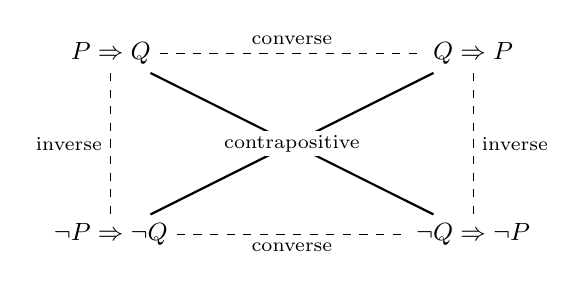
\begin{tikzpicture}[font=\small, every node/.style={inner sep=3pt}]
\node (a) at (0,2.3) {$P\Rightarrow Q$};
\node (b) at (4.6,2.3) {$Q\Rightarrow P$};
\node (c) at (0,0) {$\neg P\Rightarrow\neg Q$};
\node (d) at (4.6,0) {$\neg Q\Rightarrow\neg P$};
\draw[dashed, line width=0.4pt] (a) -- node[above, font=\scriptsize] {converse} (b);
\draw[dashed, line width=0.4pt] (c) -- node[below, font=\scriptsize] {converse} (d);
\draw[dashed, line width=0.4pt] (a) -- node[left, font=\scriptsize] {inverse} (c);
\draw[dashed, line width=0.4pt] (b) -- node[right, font=\scriptsize] {inverse} (d);
\draw[line width=0.8pt] (a) -- (d);
\draw[line width=0.8pt] (b) -- (c);
\node[font=\scriptsize, fill=white, inner sep=1.5pt] at (2.3,1.15) {contrapositive};
\end{tikzpicture}}{The four conditionals formed from $P$ and $Q$. Statements joined by a solid diagonal are contrapositives of each other and always logically equivalent; statements joined by a dashed side are not equivalent in general.\label{fig:square}}
\end{figure}

Part (ii) of \cref{prop:implication-laws} is the basis of proof by contrapositive (\cref{sec:contradiction}), and part (iii) tells us how to negate a conditional: the denial of ``if $P$, then $Q$'' is ``$P$, and yet not $Q$''. It is \emph{not} ``if $P$, then not $Q$''. Part (iv) is used when a disjunction has to be proved: to show ``$P$ or $Q$'', it suffices to assume that $P$ fails and to show that $Q$ then holds. Part (v) justifies a familiar habit of proofs, in which several hypotheses are assumed one after another.

\subsection{The Biconditional}

\begin{definition}[Biconditional]
\label{def:biconditional}
The \term{biconditional} $P\Leftrightarrow Q$, read ``$P$ if and only if $Q$'', is true when $P$ and $Q$ have the same truth value, and false otherwise.
\end{definition}

The phrase ``if and only if'' is often abbreviated to \term{iff}; the phrases ``$P$ is necessary and sufficient for $Q$'' and ``$P$ is equivalent to $Q$'' mean the same. The name is explained by the next proposition: ``$P$ if $Q$'' is $Q\Rightarrow P$, and ``$P$ only if $Q$'' is $P\Rightarrow Q$.

\begin{proposition}
\label{prop:biconditional}
For all statements $P$ and $Q$, $P\Leftrightarrow Q\equiv(P\Rightarrow Q)\wedge(Q\Rightarrow P)$. Moreover, two formulas $A$ and $B$ are logically equivalent if and only if $A\Leftrightarrow B$ is a tautology.
\end{proposition}

\begin{proof}
The conjunction $(P\Rightarrow Q)\wedge(Q\Rightarrow P)$ is false exactly when one of the two conditionals is false, that is, when $P$ is true and $Q$ false, or $Q$ true and $P$ false. These are exactly the assignments in which $P$ and $Q$ have different truth values, which by \cref{def:biconditional} are the assignments in which $P\Leftrightarrow Q$ is false (compare columns three to five of \cref{tab:truth-implication}). For the second claim, $A\Leftrightarrow B$ is true under an assignment exactly when $A$ and $B$ have the same truth value under it; so it is true under every assignment exactly when $A\equiv B$.
\end{proof}

By \cref{prop:biconditional}, a theorem of the form ``$P$ if and only if $Q$'' contains two theorems, $P\Rightarrow Q$ and $Q\Rightarrow P$, and its proof usually has two parts, often labelled ``($\Rightarrow$)'' and ``($\Leftarrow$)''. The symbols $\Leftrightarrow$ and $\equiv$ must be kept apart: the first is a connective that builds a new formula, the second is a relation between two formulas that we assert about them.

To save parentheses we agree that $\neg$ binds most tightly, then $\wedge$ and $\vee$, and then $\Rightarrow$ and $\Leftrightarrow$; thus $P\wedge Q\Rightarrow R$ means $(P\wedge Q)\Rightarrow R$. Since $\wedge$ and $\vee$ are on the same level, a formula that combines them, such as $(P\wedge Q)\vee R$, always keeps its parentheses. A chain such as $P\Rightarrow Q\Rightarrow R$ is never written without parentheses, because the two readings differ. When $P$ and $R$ are false, $P\Rightarrow(Q\Rightarrow R)$ is true, since its hypothesis is false, whereas $(P\Rightarrow Q)\Rightarrow R$ is false, since its hypothesis $P\Rightarrow Q$ is true and its conclusion $R$ is false.

\section{Predicates and Quantifiers}
\label{sec:quantifiers}

The sentence ``$x>3$'' is not a statement, because its truth depends on $x$. Yet sentences of this kind are what mathematics is made of: ``$f$ is continuous at $a$'', ``$n$ is prime'', ``$x^2-5x+6=0$''. Logic handles them by treating the variable as a slot to be filled.

\subsection{Predicates}

\begin{definition}[Predicate]
\label{def:predicate}
A \term{predicate} on a set $S$ is a sentence $P(x)$ containing a variable $x$ such that, for each element $a$ of $S$, the sentence $P(a)$ obtained by substituting $a$ for $x$ is a statement. The set $S$ is the \term{domain} of the variable, and the set $\{x\in S: P(x)\}$ of the elements for which $P(x)$ is true is the \term{truth set} of $P$.
\end{definition}

Let $P(x)$ be ``$x>3$'' on the domain $\mathbb R$. Then $P(5)$ is a true statement and $P(1)$ a false one, and the truth set of $P$ is the interval $(3,\infty)$. Predicates may have several variables. ``$x<y$'' is a predicate $P(x,y)$ in two variables; $P(1,2)$ is true and $P(2,1)$ is false. The connectives of \cref{sec:statements} apply to predicates as well: if $P(x)$ is ``$x>3$'' and $Q(x)$ is ``$x<5$'', then $P(x)\wedge Q(x)$ is ``$3<x<5$'', whose truth set is the intersection $(3,5)$ of the truth sets of $P$ and $Q$. This is the literal form of the picture of \cref{fig:venn}.

Substituting a value is one way to turn a predicate into a statement. The other way, and the more important one, is to make a claim about \emph{all} values or about \emph{some} value of the variable.

\subsection{The Universal and Existential Quantifiers}

\begin{definition}[Quantifiers]
\label{def:quantifiers}
Let $P(x)$ be a predicate on a set $S$.
\begin{enumerate}
\item The statement $\forall x\in S,\ P(x)$, read ``for every $x$ in $S$, $P(x)$'', is true if $P(a)$ is true for every element $a$ of $S$, and false otherwise. The symbol $\forall$ is the \term{universal quantifier}.
\item The statement $\exists x\in S,\ P(x)$, read ``there exists an $x$ in $S$ such that $P(x)$'', is true if $P(a)$ is true for at least one element $a$ of $S$, and false otherwise. The symbol $\exists$ is the \term{existential quantifier}.
\end{enumerate}
\end{definition}

The comma after the quantifier separates it from the formula that it governs, its \term{scope}, which extends as far to the right as the parentheses allow. When the domain is clear from the context it is sometimes omitted, as in $\forall x,\ P(x)$.

For example, $\forall x\in\mathbb R,\ x^2\ge 0$ is true, $\forall x\in\mathbb R,\ x^2>0$ is false (it fails for $x=0$), $\exists x\in\mathbb R,\ x^2=2$ is true (take $x=\sqrt2$), and $\exists x\in\mathbb Q,\ x^2=2$ is false, as we prove in \cref{sec:contradiction}. The last two examples differ only in the domain, which shows that the domain is an essential part of a quantified statement.

Programmers may recognise the quantifiers as loops. If $S$ is a finite list, $\forall x\in S,\ P(x)$ is what a loop computes that runs through $S$, returns false as soon as it finds an element failing $P$, and returns true if it reaches the end. Likewise $\exists x\in S,\ P(x)$ is computed by a loop that returns true as soon as it finds an element satisfying $P$, and false if it reaches the end. Many languages provide these two loops as library functions, commonly named \code{all} and \code{any}. For a finite domain $S=\{a_1,\ldots,a_n\}$ the quantifiers are nothing but long conjunctions and disjunctions,
\[
\forall x\in S,\ P(x)\equiv P(a_1)\wedge\cdots\wedge P(a_n),
\qquad
\exists x\in S,\ P(x)\equiv P(a_1)\vee\cdots\vee P(a_n).
\]
The quantifiers are indispensable because domains such as $\mathbb N$ and $\mathbb R$ are infinite: the loop never ends, and the truth of a universal statement over an infinite domain can be established only by an argument that applies to every element at once. Producing such arguments is what the rest of this chapter is about.

Two further remarks complete the picture. First, the variable of a quantified statement is a placeholder, like the index of a sum or the variable of integration: $\forall x\in S,\ P(x)$ and $\forall t\in S,\ P(t)$ are the same statement. Such a variable is said to be \term{bound} by the quantifier, while a variable that is not bound, like $x$ in the predicate ``$x>3$'', is \term{free}. A formula with no free variables is a statement. Second, when $S$ is empty, $\forall x\in S,\ P(x)$ is true, because no element of $S$ fails $P$, and $\exists x\in S,\ P(x)$ is false, because no element of $S$ satisfies it. This agrees with the vacuous truth of conditionals, and also with the two loops described above: on an empty list, the loop for $\forall$ reaches the end at once and returns true, and the loop for $\exists$ returns false.

A quantifier is frequently restricted to the elements satisfying a condition, as in ``for every $x>0$'' or ``there is an even $n$ such that \ldots''. Expressed with the connectives, the two restricted forms read
\begin{equation}
\forall x\in S,\ \bigl(Q(x)\Rightarrow P(x)\bigr)
\qquad\text{and}\qquad
\exists x\in S,\ \bigl(Q(x)\wedge P(x)\bigr),
\label{eq:restricted}
\end{equation}
and we abbreviate them as $\forall x\in S$ with $Q(x),\ P(x)$, or, when $Q$ is an inequality, as $\forall x>0,\ P(x)$ and $\exists x>0,\ P(x)$. The universal form uses $\Rightarrow$ and the existential form uses $\wedge$, and the difference matters. Writing $\forall x\,(Q(x)\wedge P(x))$ would claim that every $x$ satisfies $Q$, and writing $\exists x\,(Q(x)\Rightarrow P(x))$ would be satisfied by any $x$ that fails $Q$; neither is what is meant.

\subsection{Negating Quantified Statements}

To say that not every element has a property is to say that some element lacks it. This observation is used in almost every proof that involves a negation.

\begin{theorem}[Negation of quantifiers]
\label{thm:quantifier-negation}
For every predicate $P(x)$ on a set $S$,
\[
\neg\bigl(\forall x\in S,\ P(x)\bigr)\equiv\exists x\in S,\ \neg P(x)
\qquad\text{and}\qquad
\neg\bigl(\exists x\in S,\ P(x)\bigr)\equiv\forall x\in S,\ \neg P(x).
\]
\end{theorem}

Here $\equiv$ means that the two sides have the same truth value for every set $S$ and every predicate $P$, which extends \cref{def:equivalence} to quantified formulas.

\begin{proof}
By \cref{def:quantifiers}, $\forall x\in S,\ P(x)$ is false exactly when $P(a)$ is false for at least one element $a$ of $S$, that is, when $\neg P(a)$ is true for at least one $a\in S$, which is the condition for $\exists x\in S,\ \neg P(x)$ to be true. Hence the left side of the first equivalence is true exactly when the right side is.

For the second equivalence, $\exists x\in S,\ P(x)$ is false exactly when there is no element $a$ of $S$ for which $P(a)$ is true, that is, when $P(a)$ is false, and $\neg P(a)$ true, for every $a\in S$; this is the condition for $\forall x\in S,\ \neg P(x)$ to be true.
\end{proof}

For a finite domain, \cref{thm:quantifier-negation} is just De Morgan's law applied to the long conjunction and disjunction displayed above. In ordinary language the theorem guards against a common slip: the negation of ``every student passed the examination'' is ``some student did not pass'', and not ``every student failed''.

Combining \cref{thm:quantifier-negation} with De Morgan's laws and \cref{prop:implication-laws}\,(iii), any quantified statement can be negated by a mechanical procedure: move the negation inwards step by step, exchanging $\forall$ and $\exists$ each time it passes a quantifier, exchanging $\wedge$ and $\vee$ each time it passes one of them, and replacing $\neg(P\Rightarrow Q)$ by $P\wedge\neg Q$. As an example, consider the true statement that every positive real number has a real square root,
\[
\forall x\in\mathbb R,\ \bigl(x>0\Rightarrow\exists y\in\mathbb R,\ y^2=x\bigr).
\]
Its negation is transformed as follows:
\begin{align*}
\neg\Bigl(\forall x\in\mathbb R,\ \bigl(x>0\Rightarrow\exists y\in\mathbb R,\ y^2=x\bigr)\Bigr)
&\equiv\exists x\in\mathbb R,\ \neg\bigl(x>0\Rightarrow\exists y\in\mathbb R,\ y^2=x\bigr)\\
&\equiv\exists x\in\mathbb R,\ \bigl(x>0\wedge\neg\,\exists y\in\mathbb R,\ y^2=x\bigr)\\
&\equiv\exists x\in\mathbb R,\ \bigl(x>0\wedge\forall y\in\mathbb R,\ y^2\ne x\bigr).
\end{align*}
The result reads: there is a positive real number that is not the square of any real number. Exactly one of the original statement and its negation is true; in this case it is the original. Replacing $\mathbb R$ by $\mathbb Q$ in both places reverses this: the negation becomes true, with $x=2$ as a witness, because no rational number has the square $2$ (we prove this in \cref{sec:contradiction}).

\subsection{Several Quantifiers}

Statements with several variables carry several quantifiers. Quantifiers of the same kind can be exchanged freely, but quantifiers of different kinds cannot.

\begin{proposition}
\label{prop:quantifier-order}
Let $P(x,y)$ be a predicate with $x$ ranging over a set $X$ and $y$ over a set $Y$.
\begin{enumerate}
\item $\forall x\in X,\ \forall y\in Y,\ P(x,y)\equiv\forall y\in Y,\ \forall x\in X,\ P(x,y)$, and the same holds with $\exists$ in place of $\forall$.
\item If $\exists y\in Y,\ \forall x\in X,\ P(x,y)$ is true, then $\forall x\in X,\ \exists y\in Y,\ P(x,y)$ is true.
\item The converse of (ii) is false in general.
\end{enumerate}
\end{proposition}

\begin{proof}
(i) Both universal statements say that $P(a,b)$ is true for every pair $(a,b)$ with $a\in X$ and $b\in Y$, and both existential statements say that $P(a,b)$ is true for at least one such pair.

(ii) Suppose that $\exists y\in Y,\ \forall x\in X,\ P(x,y)$ is true, and choose an element $b\in Y$ such that $P(x,b)$ holds for every $x\in X$. Let $a\in X$ be arbitrary. Then $P(a,b)$ holds, so there is an element of $Y$, namely $b$, for which $P(a,y)$ holds; that is, $\exists y\in Y,\ P(a,y)$ is true. Since $a$ was arbitrary, $\forall x\in X,\ \exists y\in Y,\ P(x,y)$ is true.

(iii) Take $X=Y=\mathbb Z$ and let $P(x,y)$ be ``$y>x$''. The statement $\forall x\in\mathbb Z,\ \exists y\in\mathbb Z,\ y>x$ is true: for any integer $x$ the integer $y=x+1$ is larger. The statement $\exists y\in\mathbb Z,\ \forall x\in\mathbb Z,\ y>x$ is false: it claims an integer $y$ larger than every integer, in particular larger than itself, and $y>y$ is false.
\end{proof}

The difference between the two orders is the difference between ``everyone has someone to talk to'' and ``there is someone whom everyone talks to''. In $\forall x,\ \exists y,\ P(x,y)$ the element $y$ is chosen \emph{after} $x$ and may depend on it, as $y=x+1$ depends on $x$ in the proof of (iii). In $\exists y,\ \forall x,\ P(x,y)$ a single $y$ must serve for all $x$ at once. \Cref{fig:quantifier-grid} shows both situations for a predicate on a small finite domain, where the truth of $P(x,y)$ for every pair can be drawn as a grid of dots.

\begin{figure}
\tikzset{
  gridpanel/.pic={
    \foreach \i in {1,...,5} {
      \node[font=\scriptsize] at (\i*0.46,0.05) {$\i$};
      \node[font=\scriptsize] at (0.12,\i*0.46+0.1) {$\i$};}
    \node[font=\scriptsize] at (1.38,-0.3) {$x$};
    \node[font=\scriptsize] at (-0.2,1.48) {$y$};
    \foreach \i in {1,...,5} \foreach \j in {1,...,5}
      \draw[line width=0.3pt] (\i*0.46,\j*0.46+0.1) circle (0.055);},
  dot/.style={fill=black}}
\newcommand\gridpt[2]{\fill (#1*0.46,#2*0.46+0.1) circle (0.075);}
\sdpanel{A}{\begin{tikzpicture}
\pic {gridpanel};
\gridpt12 \gridpt14 \gridpt24 \gridpt31 \gridpt33 \gridpt45 \gridpt53 \gridpt52
\end{tikzpicture}}\hfill
\sdpanel{B}{\begin{tikzpicture}
\fill[sdfill] (0.28,3*0.46+0.1-0.17) rectangle (5*0.46+0.18,3*0.46+0.1+0.17);
\pic {gridpanel};
\gridpt13 \gridpt23 \gridpt33 \gridpt43 \gridpt53 \gridpt11 \gridpt45 \gridpt24
\end{tikzpicture}}\hfill
\sdpanel{C}{\begin{tikzpicture}
\fill[sdfill] (4*0.46-0.17,0.38) rectangle (4*0.46+0.17,5*0.46+0.28);
\pic {gridpanel};
\gridpt12 \gridpt15 \gridpt24 \gridpt31 \gridpt33 \gridpt53 \gridpt55
\end{tikzpicture}}
\caption{The order of quantifiers. Each grid shows a predicate $P(x,y)$ on $x,y\in\{1,\ldots,5\}$; a filled dot marks a pair for which $P(x,y)$ is true. (A) Every column contains a dot, so $\forall x,\ \exists y,\ P(x,y)$ is true, but no row is full, so $\exists y,\ \forall x,\ P(x,y)$ is false. (B) The shaded row $y=3$ is full, so $\exists y,\ \forall x,\ P(x,y)$ is true, and then every column contains a dot, as \cref{prop:quantifier-order}\,(ii) asserts. (C) The shaded column $x=4$ is empty, so $\forall x,\ \exists y,\ P(x,y)$ is false, and so is $\exists y,\ \forall x,\ P(x,y)$.}
\label{fig:quantifier-grid}
\end{figure}

A statement with alternating quantifiers can also be read as a game between two players. One player, the sceptic, chooses the values of the universally quantified variables and tries to make the final formula false; the other, the prover, chooses the values of the existentially quantified variables and tries to make it true. The players move in the order in which the quantifiers are written, and each sees the moves already made. The statement is true exactly when the prover has a strategy that wins against every sequence of moves by the sceptic. In $\forall x,\ \exists y,\ y>x$ the sceptic names an integer $x$ and the prover answers $x+1$, and the prover always wins. In $\exists y,\ \forall x,\ y>x$ the prover must commit to $y$ first, and the sceptic answers with $x=y$.

\subsection{Unique Existence}

Often we want to say not only that an object exists, but also that there is only one.

\begin{definition}[Unique existence]
\label{def:unique-existence}
The statement $\exists!\,x\in S,\ P(x)$, read ``there exists a unique $x$ in $S$ such that $P(x)$'', means
\[
\exists x\in S,\ \Bigl(P(x)\wedge\forall y\in S,\ \bigl(P(y)\Rightarrow y=x\bigr)\Bigr).
\]
\end{definition}

The definition says that some $x$ satisfies $P$, and that every $y$ satisfying $P$ is that same $x$. For example, $\exists!\,x\in\mathbb R,\ 2x+1=5$ is true, the unique solution being $x=2$, while $\exists!\,x\in\mathbb R,\ x^2=4$ is false, because both $2$ and $-2$ are solutions, although $\exists x\in\mathbb R,\ x^2=4$ is true. An equivalent formulation separates the two claims: $\exists!\,x\in S,\ P(x)$ holds if and only if $\exists x\in S,\ P(x)$ holds (\term{existence}) and
\[
\forall x\in S,\ \forall y\in S,\ \bigl(P(x)\wedge P(y)\Rightarrow x=y\bigr)
\]
holds (\term{uniqueness}, or ``at most one''). Proofs of unique existence almost always establish the two parts separately (\cref{sec:existence}).

\subsection{From English to Symbols}

Mathematical writing seldom uses the symbols $\forall$ and $\exists$ in running text, and it often leaves quantifiers implicit. The identity ``$x^2-1=(x-1)(x+1)$'' is a claim about every real number $x$; ``a differentiable function is continuous'' is a claim about every function; ``$\sqrt2$ is irrational'' is the claim that no pair of integers has the ratio $\sqrt2$. Before trying to prove a statement, it pays to write it with all its quantifiers explicit, because the form of the statement determines the form of the proof. \Cref{tab:translations} gives some examples.

\begin{table}
\sdfloat{%
\begin{sdtable}{colspec={Q[l,wd=4.6cm]Q[l]}, row{1}={font=\small\bfseries}}
\toprule
English & Symbols \\
\midrule
Every square of a real number is nonnegative. & $\forall x\in\mathbb R,\ x^2\ge 0$ \\
Some integer is even and prime. & $\exists n\in\mathbb Z,\ (n\text{ even}\wedge n\text{ prime})$ \\
No integer is both even and odd. & $\forall n\in\mathbb Z,\ \neg(n\text{ even}\wedge n\text{ odd})$ \\
Only zero equals its own negative. & $\forall x\in\mathbb R,\ (x=-x\Rightarrow x=0)$ \\
There is a smallest natural number. & $\exists m\in\mathbb N,\ \forall n\in\mathbb N,\ m\le n$ \\
There is no largest integer. & $\forall m\in\mathbb Z,\ \exists n\in\mathbb Z,\ n>m$ \\
Between two different real numbers there is a rational number. & $\forall x,y\in\mathbb R,\ \bigl(x<y\Rightarrow\exists q\in\mathbb Q,\ x<q<y\bigr)$ \\
\bottomrule
\end{sdtable}}{Statements in English and in symbols. The sentence ``there is no largest integer'' is translated directly into its equivalent form given by \cref{thm:quantifier-negation}.\label{tab:translations}}
\end{table}

Two of the rows deserve comment. ``No integer is both even and odd'' is literally $\neg\,\exists n\in\mathbb Z,\ (n\text{ even}\wedge n\text{ odd})$, which \cref{thm:quantifier-negation} turns into the universal form in the table. ``Only zero equals its own negative'' does not say that zero equals its own negative; it says that nothing else does. As with ``only if'', the word ``only'' points from the condition to the object.

\subsection{Reading the Definition of a Limit}

The best-known statement with alternating quantifiers in elementary mathematics is the definition of a limit, which most readers will have met in a calculus course. For a real number $t$ we write $|t|$ for its absolute value, which is $t$ if $t\ge 0$ and $-t$ if $t<0$; the number $|x-a|$ is the distance between $x$ and $a$ on the real line. The properties of the absolute value are proved in \cref{sec:direct}.

\begin{definition}[Limit of a function]
\label{def:limit}
Let $f$ be a real function defined at every point of an open interval containing the real number $a$, except possibly at $a$ itself, and let $L$ be a real number. We say that $f(x)$ \term{tends to} $L$ as $x$ tends to $a$, and write $\lim_{x\to a}f(x)=L$, if
\begin{equation}
\forall\varepsilon>0,\ \exists\delta>0,\ \forall x,\ \bigl(0<|x-a|<\delta\Rightarrow|f(x)-L|<\varepsilon\bigr),
\label{eq:limit}
\end{equation}
where $x$ ranges over the points at which $f$ is defined.
\end{definition}

This definition is discussed at length in rigorous calculus texts~\cite{spivak2008calculus}. Read as a game, it says the following. The sceptic chooses a tolerance $\varepsilon>0$, as small as desired. The prover answers with a distance $\delta>0$. The sceptic then picks any $x$ within distance $\delta$ of $a$, other than $a$ itself, and the prover wins if $f(x)$ lies within $\varepsilon$ of $L$. The limit is $L$ if the prover can always win, however small the tolerance. \Cref{fig:epsilon-delta} shows one round of the game. Three features of \eqref{eq:limit} deserve attention. First, $\delta$ comes after $\varepsilon$ and may depend on it; typically a smaller $\varepsilon$ requires a smaller $\delta$. Second, the condition $0<|x-a|$ excludes $x=a$, so the value $f(a)$, if it exists at all, has no influence on the limit. Third, the inequalities are about distances: $|f(x)-L|<\varepsilon$ says that $L-\varepsilon<f(x)<L+\varepsilon$.

\begin{figure}
\sdfloat{%
\begin{tikzpicture}
\begin{axis}[sdplot, width=6.4cm, height=5.0cm, xmin=0, xmax=3.6, ymin=0, ymax=7.5,
  xtick={1.4,2,2.6}, xticklabels={$a-\delta$,$a$,$a+\delta$},
  ytick={1.5,3,4.5}, yticklabels={$L-\varepsilon$,$L$,$L+\varepsilon$},
  xlabel={$x$}, ylabel={$f(x)$}, clip=false]
\fill[sdfill] (axis cs:0,1.5) rectangle (axis cs:3.6,4.5);
\draw[black!55, dashed, line width=0.4pt] (axis cs:1.4,0) -- (axis cs:1.4,7.5);
\draw[black!55, dashed, line width=0.4pt] (axis cs:2.6,0) -- (axis cs:2.6,7.5);
\addplot[black, line width=0.6pt, domain=0:3.6, samples=120] {1+x^2/2};
\addplot[black, line width=1.8pt, domain=1.4:2.6, samples=60] {1+x^2/2};
\draw[black, line width=0.6pt, fill=white] (axis cs:2,3) circle (2.2pt);
\end{axis}
\end{tikzpicture}}{One round of the limit game for $f(x)=1+x^2/2$, $a=2$ and $L=3$. For the tolerance $\varepsilon=1.5$ (shaded band) the distance $\delta=0.6$ works: over the interval between the dashed lines the graph (thick) stays inside the band. The open circle indicates that the value at $a$ plays no role.\label{fig:epsilon-delta}}
\end{figure}

To prove a limit, therefore, one must give a rule that produces a suitable $\delta$ for each $\varepsilon$. The following proposition is the simplest example; its proof shows the typical shape of a proof of an ``$\forall\,\exists$'' statement.

\begin{proposition}
\label{prop:limit-example}
$\lim_{x\to 2}(3x+1)=7$.
\end{proposition}

Before writing the proof, we work backwards to find $\delta$. We want $|(3x+1)-7|<\varepsilon$, and $|(3x+1)-7|=|3x-6|=3|x-2|$. So it suffices that $|x-2|<\varepsilon/3$, which suggests $\delta=\varepsilon/3$. This scratch work is not part of the proof; the proof itself runs forwards.

\begin{proof}
Let $\varepsilon>0$ be arbitrary, and put $\delta\coloneqq\varepsilon/3$, which is positive. Let $x$ be a real number with $0<|x-2|<\delta$. Then
\[
|(3x+1)-7|=3|x-2|<3\delta=\varepsilon .
\]
Since $\varepsilon$ was arbitrary, \eqref{eq:limit} holds with $f(x)=3x+1$, $a=2$ and $L=7$.
\end{proof}

The symbol $\coloneqq$ in the proof means ``is defined to be''; it introduces a new name rather than asserting an equation. The proof follows the quantifiers of \eqref{eq:limit} from left to right: ``let $\varepsilon>0$ be arbitrary'' answers $\forall\varepsilon>0$, ``put $\delta\coloneqq\varepsilon/3$'' answers $\exists\delta>0$, and ``let $x$ be a real number with \ldots'' answers $\forall x$ together with the hypothesis of the conditional.

To show that a limit is \emph{not} $L$, we negate \eqref{eq:limit} by the procedure described above:
\begin{equation}
\exists\varepsilon>0,\ \forall\delta>0,\ \exists x,\ \bigl(0<|x-a|<\delta\wedge|f(x)-L|\ge\varepsilon\bigr).
\label{eq:not-limit}
\end{equation}
In the language of the game, the sceptic has a tolerance that defeats every $\delta$ the prover might choose.

\begin{proposition}
\label{prop:step-limit}
Let $H(x)=0$ for $x<0$ and $H(x)=1$ for $x\ge 0$. Then $\lim_{x\to 0}H(x)=1$ is false.
\end{proposition}

\begin{proof}
We verify \eqref{eq:not-limit} with $a=0$ and $L=1$. Take $\varepsilon\coloneqq 1/2$. Let $\delta>0$ be arbitrary and put $x\coloneqq-\delta/2$. Then $0<|x|=\delta/2<\delta$, and since $x<0$ we have $|H(x)-1|=|0-1|=1\ge\varepsilon$.
\end{proof}

The same argument with $x=\delta/2$ shows that $\lim_{x\to 0}H(x)=0$ is false as well. In \cref{sec:existence} we show that the limit is not any number at all.

\section{The Anatomy of a Proof}
\label{sec:anatomy}

With the language in place we can say what a proof is. This section describes the kinds of statements that make up a mathematical text, the rules by which one statement may be inferred from others, and the conventions by which proofs are written and read.

\subsection{Definitions, Axioms, and Theorems}

A mathematical text consists mainly of three kinds of statements.

A \term{definition} gives a precise meaning to a word or a symbol. ``An integer $n$ is \emph{even} if $n=2k$ for some integer $k$'' is a definition. Once it is made, ``even'' means exactly this and nothing more, whatever associations the word may have in everyday language. A definition is always an ``if and only if'', even when, by long-standing custom, it is written with ``if'': an integer that is not of the form $2k$ is not even. In this book the word being defined is set in italics.

An \term{axiom} is a statement that is accepted without proof as a starting point. Every chain of reasoning must start somewhere, and the axioms are where it starts. In this chapter the axioms are the familiar properties of numbers, which we now list. They are taken for granted here and examined in \cref{ch:numbers}, where the real numbers are characterised by a short list of axioms and the other facts are derived from them.

\begin{assumption}[Arithmetic and order of numbers]
\label{asm:numbers}
We use without proof the following properties of the number systems $\mathbb N$, $\mathbb Z$, $\mathbb Q$ and $\mathbb R$, each of which contains the one before it.
\begin{enumerate}
\item The usual laws of addition, subtraction, multiplication and of division by nonzero numbers hold, together with the usual rules for inequalities; for instance, $a<b$ implies $a+c<b+c$, and $a<b$ and $c>0$ imply $ac<bc$.
\item Sums, differences and products of integers are integers. The natural numbers are the integers $n\ge 0$.
\item There is no integer $n$ with $0<n<1$. Consequently, if $m$ and $n$ are integers with $m<n$, then $m+1\le n$, since $n-m$ is a positive integer.
\item For every real number $x\ge 0$ there is exactly one real number $y\ge 0$ with $y^2=x$; it is denoted $\sqrt x$.
\end{enumerate}
\end{assumption}

A \term{theorem} is a statement that has been proved. In this book theorems come in four kinds, which differ only in their role. A \term{theorem}, in the narrow sense, is a result of central importance. A \term{proposition} is a result of lesser importance, often a building block or an example of a technique. A \term{lemma} is a result proved mainly as a step towards something else; some lemmas, once proved, turn out to be used again and again. A \term{corollary} is a result that follows quickly from a preceding theorem. All four kinds, together with definitions and assumptions, are numbered in a single sequence within each chapter, so that, for instance, \cref{def:equivalence} is followed by \cref{thm:de-morgan} and \cref{prop:laws}, and a reference to any of them can be found by its number alone. The end of every proof is marked by the symbol~\qedsymbol, set at the right margin.

The statements of a theory depend on one another: a theorem is proved from axioms, definitions and earlier results, and is then used in later proofs. \Cref{fig:dependency} shows the typical pattern. Because every proof refers only to results established before it, the whole structure rests, in the end, on the axioms and the definitions alone. This is the sense in which mathematical knowledge is cumulative, and it is also why a single error in a lemma can invalidate everything above it.

\begin{figure}
\sdfloat{%
\begin{tikzpicture}[font=\scriptsize,
  box/.style={draw, line width=0.4pt, minimum width=1.55cm, minimum height=0.52cm, inner sep=2pt},
  arr/.style={-{Latex[length=1.5mm]}, line width=0.4pt}]
\node[box, fill=sdfill] (d) at (0.1,0) {Definitions};
\node[box, fill=sdfill] (a) at (2.2,0) {Axioms};
\node[box] (l1) at (-0.85,1.15) {Lemma};
\node[box] (l2) at (3.15,1.15) {Lemma};
\node[box] (p) at (1.15,1.15) {Proposition};
\node[box, line width=0.8pt] (t) at (1.15,2.3) {Theorem};
\node[box] (c1) at (0,3.45) {Corollary};
\node[box] (c2) at (2.3,3.45) {Corollary};
\draw[arr] (d) -- (l1); \draw[arr] (d) -- (p); \draw[arr] (a) -- (p); \draw[arr] (a) -- (l2);
\draw[arr] (l1) -- (t); \draw[arr] (p) -- (t); \draw[arr] (l2) -- (t);
\draw[arr] (t) -- (c1); \draw[arr] (t) -- (c2);
\end{tikzpicture}}{The structure of a mathematical theory. An arrow from one statement to another means that the first is used in the proof of the second. Everything rests on the definitions and axioms (shaded).\label{fig:dependency}}
\end{figure}

\subsection{What a Proof Is}

A \term{proof} of a statement is a finite sequence of statements, the last of which is the statement to be proved, such that each statement in the sequence is
\begin{itemize}
\item an axiom, a hypothesis of the theorem, or a previously proved result,
\item the unfolding of a definition, or
\item a consequence of earlier statements in the sequence by a valid rule of inference.
\end{itemize}
A rule of inference is \term{valid} if it can never lead from true statements to a false one. The rules that we use are justified by tautologies, as the next proposition shows~\cite{enderton2001}.

\begin{proposition}[Rules of inference]
\label{prop:inference}
For all statements $P$, $Q$ and $R$ the following formulas are tautologies.
\begin{enumerate}
\item Modus ponens: $\bigl(P\wedge(P\Rightarrow Q)\bigr)\Rightarrow Q$.
\item Modus tollens: $\bigl(\neg Q\wedge(P\Rightarrow Q)\bigr)\Rightarrow\neg P$.
\item Chaining: $\bigl((P\Rightarrow Q)\wedge(Q\Rightarrow R)\bigr)\Rightarrow(P\Rightarrow R)$.
\item Cases: $\bigl((P\Rightarrow R)\wedge(Q\Rightarrow R)\bigr)\Rightarrow\bigl((P\vee Q)\Rightarrow R\bigr)$.
\item Contradiction: $\bigl(\neg P\Rightarrow(R\wedge\neg R)\bigr)\Rightarrow P$.
\end{enumerate}
\end{proposition}

Instead of writing out truth tables, we use a shortcut that is itself an argument by contradiction (\cref{sec:contradiction}). A conditional is false only when its hypothesis is true and its conclusion is false; so to show that a conditional is a tautology, we suppose that some assignment makes the hypothesis true and the conclusion false, and we show that no such assignment exists.

\begin{proof}
(i) Suppose that an assignment makes $Q$ false and both $P$ and $P\Rightarrow Q$ true. With $P$ true and $Q$ false, $P\Rightarrow Q$ is false, which is impossible.

(ii) By \cref{prop:implication-laws}\,(ii), $P\Rightarrow Q\equiv\neg Q\Rightarrow\neg P$, so (ii) is (i) applied to $\neg Q$ and $\neg P$.

(iii) Suppose that an assignment makes $P\Rightarrow R$ false, that is, $P$ true and $R$ false, while $P\Rightarrow Q$ and $Q\Rightarrow R$ are true. Since $P$ is true and $P\Rightarrow Q$ is true, $Q$ is true; since $Q$ is true and $Q\Rightarrow R$ is true, $R$ is true. This contradicts the assumption that $R$ is false.

(iv) Suppose that an assignment makes $P\vee Q$ true and $R$ false, while $P\Rightarrow R$ and $Q\Rightarrow R$ are true. As $R$ is false and $P\Rightarrow R$ is true, $P$ must be false; likewise $Q$ must be false. Then $P\vee Q$ is false, a contradiction.

(v) Suppose that an assignment makes $P$ false and $\neg P\Rightarrow(R\wedge\neg R)$ true. Then $\neg P$ is true, so $R\wedge\neg R$ is true, which is impossible by \cref{prop:laws}\,(vii).
\end{proof}

Each rule corresponds to a way of reasoning. Modus ponens is the basic step of every proof: we know $P$, we know that $P$ implies $Q$, and so we know $Q$. Chaining allows a long argument to be assembled from short steps. The rule of cases is the basis of proof by cases (\cref{sec:direct}), modus tollens and the contrapositive are the basis of proof by contrapositive, and the last rule is the basis of proof by contradiction (\cref{sec:contradiction}).

Two further rules concern quantifiers, and they are used in almost every proof in this book.
\begin{itemize}
\item To prove $\forall x\in S,\ P(x)$, let $x$ be an \emph{arbitrary} element of $S$, about which nothing is assumed except that it belongs to $S$, and prove $P(x)$. Since the argument used no property of $x$ beyond membership in $S$, it applies equally to every element of $S$. The step ``let $a\in X$ be arbitrary'' in the proof of \cref{prop:quantifier-order}\,(ii) and the first line of the proof of \cref{prop:limit-example} are of this kind.
\item To prove $\exists x\in S,\ P(x)$, it suffices to exhibit one element $a$ of $S$ and prove $P(a)$. Conversely, when $\exists x\in S,\ P(x)$ is known, we may give a name to one such element and use it, as long as we assume nothing about it except that it lies in $S$ and satisfies $P$.
\end{itemize}

Proofs in mathematical texts, including this one, are written in prose rather than as numbered sequences of statements, and they omit steps that a reader with the necessary background can supply. The standard is this: a proof is complete if every competent reader can fill in the omitted steps without new ideas. What counts as a routine step depends on the reader, and in this chapter we omit very little. Formal proofs, in which no step at all is omitted, are a subject of their own; the note at the end of this section describes them briefly.

\subsection{Finding the Hypothesis and the Conclusion}

The first step towards a proof is to identify exactly what is assumed and what must be shown. Most theorems can be brought to the form
\[
\forall x\in S,\ \bigl(H(x)\Rightarrow C(x)\bigr),
\]
where $H(x)$ is the hypothesis and $C(x)$ the conclusion, possibly after expanding hidden quantifiers. ``The sum of two odd integers is even'' becomes: for all integers $m$ and $n$, if $m$ and $n$ are odd, then $m+n$ is even. ``A differentiable function is continuous'' becomes: for every function $f$ and every point $a$, if $f$ is differentiable at $a$, then $f$ is continuous at $a$. After this translation, the general rules dictate the first lines of the proof: let $x\in S$ be arbitrary, assume $H(x)$, and work towards $C(x)$.

During a proof it helps to keep two lists in mind: the \term{givens}, which are the facts available at the moment, and the \term{goal}, which is the statement that remains to be proved~\cite{velleman2019}. Each step of the proof either adds to the givens or replaces the goal by a simpler one. \Cref{tab:givens-goal} shows the lists during the proof of the following proposition, which is the claim \eqref{eq:n-greater-two} of \cref{sec:implication}, now for real numbers.

\begin{proposition}
\label{prop:x-greater-two}
For every real number $x$, if $x>2$, then $x^2>4$.
\end{proposition}

\begin{proof}
Let $x$ be a real number with $x>2$. Then $x>0$, and multiplying the inequality $x>2$ by the positive number $x$ gives $x^2>2x$. Multiplying $x>2$ by $2$ gives $2x>4$. Hence $x^2>2x>4$.
\end{proof}

\begin{table}
\sdfloat{%
\begin{sdtable}{colspec={Q[l,wd=2.9cm]Q[l,wd=3.0cm]Q[l,wd=3.9cm]}, row{1}={font=\small\bfseries}}
\toprule
Step & New givens & Goal \\
\midrule
start & none & $\forall x\in\mathbb R,\ (x>2\Rightarrow x^2>4)$ \\
let $x\in\mathbb R$ be arbitrary & $x\in\mathbb R$ & $x>2\Rightarrow x^2>4$ \\
assume the hypothesis & $x>2$ & $x^2>4$ \\
derive consequences & $x>0$, $x^2>2x$, $2x>4$ & $x^2>4$ \\
chain the inequalities & $x^2>4$ & reached \\
\bottomrule
\end{sdtable}}{Givens and goal during the proof of \cref{prop:x-greater-two}. Each row lists the givens added at that step; the earlier givens remain available. The steps ``let'' and ``assume'' are dictated by the form of the statement; only the derivation of consequences requires an idea.\label{tab:givens-goal}}
\end{table}

The table shows how little of a typical proof requires an idea. Introducing $x$ and assuming the hypothesis are dictated by the logical form of the statement; only the step ``multiply by $x$'' needs insight. As statements grow more complex, the form dictates more and more of the proof, and recognising the form is a large part of the skill of proving theorems. P\'olya's classic book~\cite{polya1945} discusses the other part, finding the ideas, at length.

\subsection{The Language of Proofs}

Proofs use a small vocabulary of set phrases, each with a precise logical role.
\begin{itemize}
\item ``Let $x$ be \ldots'' introduces an arbitrary element, in preparation for proving a universal statement. ``Suppose'' or ``assume'' introduces a hypothesis, which remains available until the end of the argument that it opens.
\item ``Then'', ``hence'', ``therefore'', ``so'' and ``it follows that'' announce a statement derived from earlier ones. A good proof makes it clear which earlier statements are used.
\item ``We must show that'' or ``it suffices to show that'' announces a change of goal. ``It suffices to show $Q$'' means that $Q$ implies the current goal, so proving $Q$ completes the proof.
\item ``Without loss of generality'' announces that only one of several cases will be treated, because the others are the same up to renaming. It is legitimate only when the claim is symmetric, for example under the exchange of $x$ and $y$.
\item ``Choose'' or ``put'', often with $\coloneqq$, gives a name to a specific object, such as the $\delta$ in the proof of \cref{prop:limit-example}.
\end{itemize}

\begin{note}{Formal proofs and the limits of proof}
In mathematical logic a proof is a formal object: a finite sequence of formulas in a fixed symbolic language, each obtained from earlier ones by a fixed list of rules, so that checking a proof is a purely mechanical task~\cite{enderton2001}. Computer programs called proof assistants perform this check, and substantial parts of mathematics have been formalised with them: complete machine-checked proofs exist, for example, of the odd order theorem of finite group theory~\cite{gonthier2013oddorder} and of the Kepler conjecture on the densest packing of spheres~\cite{hales2017kepler}, and the library mathlib of the Lean proof assistant collects a large body of formalised mathematics~\cite{mathlib2020}. Two theorems of Kurt G\"odel describe what formal proof can and cannot do. The completeness theorem~\cite{godel1930} states that in first-order logic, the logic of the quantifiers $\forall$ and $\exists$ over a single domain, every statement that is true in every structure satisfying a set of axioms has a formal proof from those axioms. The incompleteness theorem~\cite{godel1931}, in the form later strengthened by Rosser~\cite{rosser1936}, states that any consistent system of axioms that can be listed by a computer program and that includes the basic arithmetic of $\mathbb N$ leaves some statements about natural numbers that it can neither prove nor refute. Neither theorem affects the everyday practice of mathematics described in this chapter, but together they show that ``true'' and ``provable'' are different notions.
\end{note}

\section{Direct Proof and Proof by Cases}
\label{sec:direct}

The simplest way to prove a conditional $P\Rightarrow Q$ is to assume $P$ and to deduce $Q$ by a chain of valid steps; by the rule of chaining in \cref{prop:inference}, the chain then establishes $P\Rightarrow Q$. Such a proof is called a \term{direct proof}. \Cref{prop:limit-example,prop:x-greater-two} were proved directly. This section develops the technique with examples from the arithmetic of integers, where the definitions are simple and the arguments are short, and then adds the technique of splitting a proof into cases.

\subsection{Even and Odd Integers}

\begin{definition}[Even, odd, divisibility]
\label{def:even-odd}
An integer $n$ is \term{even} if there is an integer $k$ with $n=2k$, and \term{odd} if there is an integer $k$ with $n=2k+1$. For integers $a$ and $b$, we say that $a$ \term{divides} $b$, or that $b$ is a \term{multiple} of $a$, and write $a\mid b$, if there is an integer $k$ with $b=ak$.
\end{definition}

Thus $0=2\cdot0$ is even, $-7=2\cdot(-4)+1$ is odd, $3\mid 12$, $-3\mid 12$ and $5\mid 0$. Every integer divides $0$, while $0$ divides only $0$. An integer is even exactly when $2$ divides it. The expression $a\mid b$ is a statement, true or false, while $a/b$ is a number; the two must not be confused.

The following proposition is intuitively obvious, and we shall use it throughout. We prove it in \cref{sec:induction}, once mathematical induction is available.

\begin{proposition}[Parity]
\label{prop:parity}
Every integer is either even or odd, and no integer is both.
\end{proposition}

The first direct proofs combine \cref{def:even-odd} with algebra. We prove two parts of the following proposition in detail; the others are proved in the same way.

\begin{proposition}
\label{prop:even-odd-arith}
Let $m$ and $n$ be integers.
\begin{enumerate}
\item If $m$ and $n$ are both even or both odd, then $m+n$ is even.
\item If one of $m$ and $n$ is even and the other is odd, then $m+n$ is odd.
\item If $m$ is even, then $mn$ is even.
\item If $m$ and $n$ are both odd, then $mn$ is odd.
\end{enumerate}
\end{proposition}

Let us think through part (i) for two odd integers before writing anything. The hypothesis says that $m$ and $n$ are odd; by \cref{def:even-odd} this means that $m=2k+1$ and $n=2l+1$ for some integers $k$ and $l$. The goal is that $m+n$ is even, which by the same definition means that $m+n=2j$ for some integer $j$. So we compute $m+n$ and look for a factor $2$. The only point that needs care is that $m$ and $n$ may be different numbers, so the two integers $k$ and $l$ must get different names.

\begin{proof}
(i) Suppose first that $m$ and $n$ are odd, say $m=2k+1$ and $n=2l+1$ with integers $k$ and $l$. Then
\[
m+n=2k+1+2l+1=2(k+l+1),
\]
and $k+l+1$ is an integer by \cref{asm:numbers}\,(ii), so $m+n$ is even. If $m=2k$ and $n=2l$ are both even, then $m+n=2(k+l)$ is even.

(iv) Suppose that $m=2k+1$ and $n=2l+1$ with integers $k$ and $l$. Then
\[
mn=(2k+1)(2l+1)=4kl+2k+2l+1=2(2kl+k+l)+1,
\]
and $2kl+k+l$ is an integer, so $mn$ is odd.

Parts (ii) and (iii) are proved in the same way: if $m=2k$ and $n=2l+1$, then $m+n=2(k+l)+1$; and if $m=2k$, then $mn=2(kn)$.
\end{proof}

Divisibility behaves in a similarly simple way.

\begin{proposition}
\label{prop:divisibility}
Let $a$, $b$ and $c$ be integers.
\begin{enumerate}
\item $a\mid a$ and $1\mid a$.
\item If $a\mid b$ and $b\mid c$, then $a\mid c$.
\item If $a\mid b$ and $a\mid c$, then $a\mid(bx+cy)$ for all integers $x$ and $y$.
\item If $a\mid b$ and $b\ne0$, then $|a|\le|b|$.
\end{enumerate}
\end{proposition}

\begin{proof}
(i) $a=a\cdot1$ and $a=1\cdot a$.

(ii) By hypothesis there are integers $k$ and $l$ with $b=ak$ and $c=bl$. Then $c=(ak)l=a(kl)$, and $kl$ is an integer, so $a\mid c$.

(iii) Write $b=ak$ and $c=al$ with integers $k$ and $l$, and let $x$ and $y$ be arbitrary integers. Then $bx+cy=akx+aly=a(kx+ly)$, and $kx+ly$ is an integer.

(iv) Write $b=ak$. Since $b\ne0$, also $k\ne0$, so $|k|\ge1$ by \cref{asm:numbers}\,(iii), and $|b|=|a|\,|k|\ge|a|$, using the rule $|xy|=|x|\,|y|$ proved below in \cref{prop:abs}.
\end{proof}

A slightly longer chain of steps gives a less obvious fact about odd squares. For instance, $3^2-1=8$, $5^2-1=24$ and $7^2-1=48$ are all multiples of $8$.

\begin{proposition}
\label{prop:odd-square}
If $n$ is an odd integer, then $8\mid n^2-1$.
\end{proposition}

\begin{proof}
Write $n=2k+1$ with an integer $k$. Then $n^2-1=4k^2+4k=4k(k+1)$. By \cref{prop:consecutive} below, $k(k+1)$ is even, say $k(k+1)=2j$ with an integer $j$. Hence $n^2-1=8j$.
\end{proof}

The proof used a fact, that the product of two consecutive integers is even, which we prove next by a new technique.

\subsection{Proof by Cases}

Sometimes a single argument does not cover all situations, but the situations can be divided into a few cases, each of which can be handled separately. If every situation falls into at least one of the cases, and the conclusion is proved in each case, then the conclusion holds in every situation. This is the rule of cases of \cref{prop:inference}\,(iv): from $P\Rightarrow R$ and $Q\Rightarrow R$ we may infer $(P\vee Q)\Rightarrow R$, and if $P\vee Q$ is known to hold, then $R$ follows. The cases need not exclude one another, but together they must be \term{exhaustive}: forgetting a case is the typical error of this technique.

\begin{proposition}
\label{prop:consecutive}
For every integer $n$, the product $n(n+1)$ is even.
\end{proposition}

\begin{proof}
By \cref{prop:parity}, $n$ is even or odd, and we treat the two cases separately.

\emph{Case 1: $n$ is even.} Then $n(n+1)$ is even by \cref{prop:even-odd-arith}\,(iii).

\emph{Case 2: $n$ is odd.} Then $n+1$ is even by \cref{prop:even-odd-arith}\,(i), since $1$ is odd. Hence $n(n+1)=(n+1)n$ is even by \cref{prop:even-odd-arith}\,(iii).

The two cases exhaust all integers, so $n(n+1)$ is even for every integer $n$.
\end{proof}

The absolute value is defined by cases, so it is natural that its properties are proved by cases. These properties are used constantly in analysis and in numerical computation, where errors are measured by absolute values~\cite{spivak2008calculus}.

\begin{proposition}[Absolute value]
\label{prop:abs}
For all real numbers $x$, $y$ and every real number $c\ge0$:
\begin{enumerate}
\item $|x|\ge0$, $|-x|=|x|$ and $-|x|\le x\le|x|$;
\item $|xy|=|x|\,|y|$;
\item $|x|\le c$ if and only if $-c\le x\le c$, and likewise with $<$ in both places;
\item the triangle inequality $|x+y|\le|x|+|y|$ holds.
\end{enumerate}
\end{proposition}

\begin{proof}
(i) If $x\ge0$, then $|x|=x\ge0$, $|-x|=-(-x)=x$ because $-x\le0$ (when $x=0$ both definitions give $0$), and $-|x|=-x\le0\le x=|x|$. If $x<0$, then $|x|=-x>0$, $|-x|=-x=|x|$ because $-x>0$, and $-|x|=x<0<-x=|x|$. In both cases all three claims hold.

(ii) We consider the signs of $x$ and $y$. If $x\ge0$ and $y\ge0$, then $xy\ge0$ and $|xy|=xy=|x|\,|y|$. If $x\ge0$ and $y<0$, then $xy\le0$ and $|xy|=-xy=x(-y)=|x|\,|y|$. The case $x<0\le y$ is the same with $x$ and $y$ exchanged, and if $x<0$ and $y<0$, then $xy>0$ and $|xy|=xy=(-x)(-y)=|x|\,|y|$.

(iii) Suppose $|x|\le c$. By (i), $x\le|x|\le c$ and $-c\le-|x|\le x$. Conversely, suppose $-c\le x\le c$. If $x\ge0$, then $|x|=x\le c$; if $x<0$, then $|x|=-x\le c$, because $-c\le x$. The version with strict inequalities is proved in the same way.

(iv) By (i), $-|x|\le x\le|x|$ and $-|y|\le y\le|y|$. Adding these inequalities gives
\[
-(|x|+|y|)\le x+y\le|x|+|y|,
\]
and (iii) with $c=|x|+|y|$ yields $|x+y|\le|x|+|y|$.
\end{proof}

The proof of (iv) shows that cases, once used to establish a basic fact such as (i) or (iii), need not be repeated: the triangle inequality follows from (i) and (iii) by a direct argument. A proof by cases on the signs of $x$, $y$ and $x+y$ is also possible but longer. \Cref{fig:triangle} illustrates the content of the triangle inequality on the real line: the distance from $0$ to $x+y$ is at most the length of the path from $0$ to $x$ and on to $x+y$, with equality when the two steps go in the same direction.

\begin{figure}
\tikzset{nl/.style={line width=0.4pt}, tstep/.style={-{Latex[length=1.6mm]}, line width=0.7pt}}
\sdpanel{A}{\begin{tikzpicture}[font=\scriptsize]
\draw[nl] (-0.3,0) -- (5.0,0);
\foreach \p/\l in {0/$0$, 2.2/$x$, 3.8/$x+y$} {\draw[nl] (\p,-0.07) -- (\p,0.07); \node[below] at (\p,-0.07) {\l};}
\draw[tstep] (0,0.32) -- node[above] {$|x|$} (2.2,0.32);
\draw[tstep] (2.2,0.32) -- node[above] {$|y|$} (3.8,0.32);
\draw[tstep, black!50] (0,1.55) -- node[above, black] {$|x+y|$} (3.8,1.55);
\end{tikzpicture}}\hfill
\sdpanel{B}{\begin{tikzpicture}[font=\scriptsize]
\draw[nl] (-0.3,0) -- (5.0,0);
\foreach \p/\l in {0/$0$, 3.6/$x$, 1.6/$x+y$} {\draw[nl] (\p,-0.07) -- (\p,0.07); \node[below] at (\p,-0.07) {\l};}
\draw[tstep] (0,0.32) -- node[above] {$|x|$} (3.6,0.32);
\draw[tstep] (3.6,0.95) -- node[above] {$|y|$} (1.6,0.95);
\draw[tstep, black!50] (0,1.55) -- node[above, black] {$|x+y|$} (1.6,1.55);
\end{tikzpicture}}
\caption{The triangle inequality on the real line. (A) When $x$ and $y$ have the same sign, the steps $x$ and $y$ point the same way and $|x+y|=|x|+|y|$. (B) When they have opposite signs, the second step turns back and $|x+y|<|x|+|y|$.}
\label{fig:triangle}
\end{figure}

A consequence that is often needed bounds the difference of two absolute values; it is called the reverse triangle inequality.

\begin{corollary}[Reverse triangle inequality]
\label{cor:reverse-triangle}
For all real numbers $x$ and $y$, $\bigl||x|-|y|\bigr|\le|x-y|$.
\end{corollary}

\begin{proof}
By the triangle inequality, $|x|=|(x-y)+y|\le|x-y|+|y|$, so $|x|-|y|\le|x-y|$. Exchanging $x$ and $y$ gives $|y|-|x|\le|y-x|=|x-y|$, using $|-t|=|t|$. Thus $-|x-y|\le|x|-|y|\le|x-y|$, and \cref{prop:abs}\,(iii) gives the claim.
\end{proof}

Cases also appear in formulas that avoid them. The following identity expresses the maximum of two numbers, which is defined by cases, by a single formula.

\begin{proposition}
\label{prop:max}
For all real numbers $a$ and $b$, $\max(a,b)=\tfrac12\bigl(a+b+|a-b|\bigr)$, where $\max(a,b)$ is $a$ if $a\ge b$ and $b$ otherwise.
\end{proposition}

\begin{proof}
If $a\ge b$, then $|a-b|=a-b$ and the right side is $\tfrac12(a+b+a-b)=a=\max(a,b)$. If $a<b$, then $|a-b|=-(a-b)=b-a$ and the right side is $\tfrac12(a+b+b-a)=b=\max(a,b)$.
\end{proof}

The expression $\tfrac12(a+b+|a-b|)$ is symmetric in $a$ and $b$, and so is $\max(a,b)$. In such a situation one often writes ``without loss of generality, $a\ge b$'' and treats only the first case: the second case is the first with the names $a$ and $b$ exchanged, and exchanging the names changes neither side of the identity.

\section{Contrapositive and Contradiction}
\label{sec:contradiction}

A direct proof works forwards from the hypothesis. Some statements resist this approach, typically because the hypothesis or the conclusion is negative (``$x$ is irrational'', ``$n$ is not prime'', ``there is no largest \ldots'') and a negative statement gives nothing concrete to compute with. The two techniques of this section turn such statements around.

\subsection{Proof by Contrapositive}

By \cref{prop:implication-laws}\,(ii), a conditional $P\Rightarrow Q$ is logically equivalent to its contrapositive $\neg Q\Rightarrow\neg P$. Hence, to prove $P\Rightarrow Q$, we may instead assume $\neg Q$ and deduce $\neg P$ directly. This is a \term{proof by contrapositive}. It is useful when $\neg Q$ is a more convenient starting point than $P$.

\begin{proposition}
\label{prop:square-even}
Let $n$ be an integer. If $n^2$ is even, then $n$ is even. If $n^2$ is odd, then $n$ is odd.
\end{proposition}

A direct attempt at the first claim starts from $n^2=2k$ and must somehow extract information about $n$ itself, for which there is no obvious way, since $\sqrt{2k}$ need not be an integer. The contrapositive starts from information about $n$ and asks about $n^2$, which only requires squaring.

\begin{proof}
We prove the contrapositive of the first claim: if $n$ is not even, then $n^2$ is not even. Suppose $n$ is not even. By \cref{prop:parity}, $n$ is odd, so $n^2=n\cdot n$ is odd by \cref{prop:even-odd-arith}\,(iv), and by \cref{prop:parity} again it is not even.

For the second claim, suppose that $n$ is not odd. Then $n$ is even by \cref{prop:parity}, so $n^2$ is even by \cref{prop:even-odd-arith}\,(iii), hence not odd.
\end{proof}

The next example involves rational numbers, which we now define, together with their opposites.

\begin{definition}[Rational and irrational numbers]
\label{def:rational}
A real number $x$ is \term{rational} if there are integers $p$ and $q$ with $q\ne0$ and $x=p/q$. A real number that is not rational is \term{irrational}. A fraction $p/q$ is in \term{lowest terms} if $q>0$ and no integer $d\ge2$ divides both $p$ and $q$.
\end{definition}

If $x=p/q$ and $y=r/s$ are rational, then $x+y=(ps+rq)/(qs)$, $x-y=(ps-rq)/(qs)$ and $xy=(pr)/(qs)$ with $qs\ne0$, so sums, differences and products of rational numbers are rational; so are quotients by nonzero rational numbers.

\begin{proposition}
\label{prop:sqrt-irrational}
Let $x>0$ be a real number. If $x$ is irrational, then $\sqrt x$ is irrational.
\end{proposition}

\begin{proof}
We prove the contrapositive: if $\sqrt x$ is rational, then $x$ is rational. Suppose $\sqrt x=p/q$ with integers $p$ and $q\ne0$. Then $x=(\sqrt x)^2=p^2/q^2$, where $p^2$ and $q^2\ne0$ are integers, so $x$ is rational.
\end{proof}

Again the contrapositive replaces a negative hypothesis (``$x$ is irrational'', which says only what $x$ is not) by a positive one (``$\sqrt x=p/q$'', which can be squared).

\subsection{Proof by Contradiction}

A \term{proof by contradiction} establishes a statement $P$ by assuming $\neg P$ and deducing a contradiction, that is, a statement of the form $R\wedge\neg R$. The justification is the last rule of \cref{prop:inference}: if $\neg P$ implies something impossible, then $\neg P$ is false and $P$ is true. To prove a conditional $P\Rightarrow Q$ by contradiction, one assumes its negation, which by \cref{prop:implication-laws}\,(iii) is $P\wedge\neg Q$, and derives a contradiction. In other words, one assumes the hypothesis and the denial of the conclusion together. The statement $R$ that leads to the contradiction is not given in advance; finding it is part of the proof.

The standard first example of a proof by contradiction is the irrationality of $\sqrt2$, a fact known to the mathematicians of ancient Greece~\cite{hardywright2008}. The proof needs one auxiliary fact about fractions, which we prove in \cref{sec:induction} with the well-ordering principle.

\begin{lemma}[Lowest terms]
\label{lem:lowest-terms}
Every rational number can be written as a fraction in lowest terms.
\end{lemma}

\begin{theorem}
\label{thm:sqrt2}
The number $\sqrt2$ is irrational.
\end{theorem}

\begin{proof}
Suppose, for a contradiction, that $\sqrt2$ is rational. By \cref{lem:lowest-terms} we can write $\sqrt2=p/q$ in lowest terms, so that $q>0$ and no integer $d\ge2$ divides both $p$ and $q$. Squaring and multiplying by $q^2$ gives
\[
p^2=2q^2 .
\]
Hence $p^2$ is even, and $p$ is even by \cref{prop:square-even}; write $p=2k$ with an integer $k$. Substituting, $4k^2=2q^2$, that is, $q^2=2k^2$. Hence $q^2$ is even, and $q$ is even by \cref{prop:square-even}. Thus $2$ divides both $p$ and $q$, which contradicts the choice of $p/q$ in lowest terms. Therefore $\sqrt2$ is irrational.
\end{proof}

It follows that no rational number $x$ satisfies $x^2=2$, as claimed in \cref{sec:quantifiers}: for such an $x$ we would have $|x|\ge0$ and $|x|^2=x^2=2$, so $|x|=\sqrt2$ by \cref{asm:numbers}\,(iv), and $|x|$, which is $x$ or $-x$, would be rational.

In this proof $R$ is the statement ``some integer $d\ge2$ divides both $p$ and $q$''. The choice of a fraction in lowest terms gives $\neg R$, and the computation gives $R$. \Cref{fig:contradiction} sets the general pattern beside this instance. By \cref{prop:sqrt-irrational}, the irrationality of $\sqrt2$ also gives the irrationality of $\sqrt{\sqrt2}=2^{1/4}$, $2^{1/8}$, and so on.

\begin{figure}
\sdfloat{%
\begin{tikzpicture}[font=\scriptsize,
  st/.style={draw, line width=0.4pt, rounded corners=2pt, text width=3.9cm, align=flush left, inner sep=3pt, minimum height=0.62cm},
  arr/.style={-{Latex[length=1.5mm]}, line width=0.4pt}]
\node[font=\small\bfseries] at (0,0.55) {Pattern};
\node[font=\small\bfseries] at (5.1,0.55) {Instance: $\sqrt2$};
\foreach \y/\l/\r [count=\i] in {
  0/{Goal: prove $P$.}/{Goal: $\sqrt2$ is irrational.},
  -1.05/{Assume $\neg P$.}/{Assume $\sqrt2=p/q$ in lowest terms.},
  -2.1/{Deduce consequences from $\neg P$ and known results.}/{$p^2=2q^2$, so $p$ is even; then $q^2=2k^2$, so $q$ is even.},
  -3.15/{Reach a statement $R$ and its negation $\neg R$.}/{$2$ divides $p$ and $q$, yet $p/q$ is in lowest terms.},
  -4.2/{Conclude that $\neg P$ is false, so $P$ is true.}/{$\sqrt2$ is irrational.}} {
  \node[st, fill=sdfill] (l\i) at (0,\y) {\l};
  \node[st] (r\i) at (5.1,\y) {\r};
  \draw[line width=0.3pt, dotted] (l\i) -- (r\i);}
\foreach \i/\j in {1/2,2/3,3/4,4/5} {\draw[arr] (l\i) -- (l\j); \draw[arr] (r\i) -- (r\j);}
\end{tikzpicture}}{The structure of a proof by contradiction (left) and its instance in the proof of \cref{thm:sqrt2} (right).\label{fig:contradiction}}
\end{figure}

A second example of the same age is Euclid's theorem on prime numbers, which appears as Proposition~20 of Book~IX of the \emph{Elements}~\cite{heath1956euclid} and has since been proved in many other ways~\cite{aigner2018proofs,hardywright2008}.

\begin{definition}[Prime number]
\label{def:prime}
An integer $p\ge2$ is \term{prime} if its only positive divisors are $1$ and $p$. An integer $n\ge2$ that is not prime is \term{composite}.
\end{definition}

The first primes are $2,3,5,7,11,13$. By \cref{prop:divisibility}\,(iv), a positive divisor $d$ of an integer $n\ge2$ satisfies $1\le d\le n$, so $n$ is composite exactly when it has a divisor $d$ with $1<d<n$. The proof of Euclid's theorem uses the following lemma, whose proof by strong induction is given in \cref{sec:induction}.

\begin{lemma}[Prime divisor]
\label{lem:prime-divisor}
Every integer $n\ge2$ has a prime divisor.
\end{lemma}

``There are infinitely many primes'' has to be given a precise meaning before it can be proved. We take it to mean that no finite list contains all primes, which is the form in which Euclid stated it.

\begin{theorem}[Euclid]
\label{thm:euclid}
There are infinitely many prime numbers: for every finite list $p_1,\ldots,p_k$ of primes there is a prime that is not in the list.
\end{theorem}

\begin{proof}
Let $p_1,\ldots,p_k$ be primes, and suppose, for a contradiction, that every prime is in the list. Consider
\[
N\coloneqq p_1p_2\cdots p_k+1 .
\]
Since every $p_i\ge2$ (and an empty product equals $1$), we have $N\ge2$, so by \cref{lem:prime-divisor} $N$ has a prime divisor $p$. By our assumption, $p$ is one of $p_1,\ldots,p_k$, so $p$ divides the product $M\coloneqq p_1p_2\cdots p_k$. Since $p$ divides both $N$ and $M$, it divides $N-M=1$ by \cref{prop:divisibility}\,(iii) with $x=1$ and $y=-1$. But then $p\le1$ by \cref{prop:divisibility}\,(iv), contradicting $p\ge2$. Hence some prime is not in the list.
\end{proof}

A common misreading of this proof is that $N=p_1\cdots p_k+1$ is itself always prime. It is not: $2\cdot3\cdot5\cdot7\cdot11\cdot13+1=30031=59\cdot509$. The proof shows only that the prime divisors of $N$ lie outside the list; here they are $59$ and $509$.

Here is a third example, in which the contradiction is reached in a single step.

\begin{proposition}
\label{prop:no-smallest}
There is no smallest positive real number.
\end{proposition}

\begin{proof}
Suppose, for a contradiction, that $\varepsilon$ is a smallest positive real number. Then $\varepsilon/2$ is a real number with $0<\varepsilon/2<\varepsilon$, so it is positive and smaller than $\varepsilon$. This contradicts the choice of $\varepsilon$.
\end{proof}

The proposition is a statement about real numbers and not about the numbers in a computer. The binary64 floating-point format used by almost all scientific software contains a smallest positive number, $2^{-1074}\approx4.9\times10^{-324}$, and halving it gives zero under the default rounding rule~\cite{ieee754-2019}. Facts about $\mathbb R$ hold for floating-point numbers only when they have been proved for them; Volume~V of this series is devoted to such proofs.

\subsection{Choosing Between the Techniques}

Every proof by contrapositive can be read as a proof by contradiction: assuming $P$ and $\neg Q$, the contrapositive argument derives $\neg P$ from $\neg Q$, and $P\wedge\neg P$ is a contradiction. Conversely, many proofs by contradiction can be reorganised as direct proofs or as proofs by contrapositive, and when this is possible the reorganised proof is usually better. In a proof by contradiction, every statement after the initial assumption is a statement about a situation that does not exist; such statements cannot be checked on examples, and a mistake among them is harder to notice. A direct proof or a proof by contrapositive, by contrast, consists of true statements throughout, which can be reused elsewhere. Proof by contradiction remains indispensable when the claim is itself a negative statement, such as ``$\sqrt2$ is not rational'' or ``there is no smallest positive real number'', because then the assumption $\neg P$ is the only concrete object to work with.

\section{Mathematical Induction}
\label{sec:induction}

Many statements in this book are claims about every natural number: a formula for a sum of $n$ terms, an error bound after $n$ steps of an algorithm, a property of matrices of every size $n$. Such a claim consists of infinitely many statements $P(0)$, $P(1)$, $P(2)$, \ldots, and checking them one at a time never ends. Mathematical induction proves them all with two finite arguments.

\subsection{The Principle of Induction}

Imagine an endless row of dominoes standing on end, numbered $0$, $1$, $2$, \ldots, and suppose two things: the first domino is pushed over, and the dominoes are spaced so that whenever one falls, it knocks over the next. Then every domino falls. Domino number $1000$ falls because number $999$ does, which falls because number $998$ does, and so on back to the first. \Cref{fig:dominoes} shows the picture, together with what happens when the spacing is wrong at one place.

\begin{figure}
\tikzset{
  domino/.style={fill=sdfill, draw=black, line width=0.4pt},
  hit/.style={-{Latex[length=1.4mm]}, line width=0.4pt, bend left=50}}
\sdpanel{A}{\begin{tikzpicture}[font=\scriptsize]
\draw[line width=0.4pt] (-0.5,0) -- (10.6,0);
\begin{scope}[rotate around={-24:(0.4,0)}]\draw[domino] (0.2,0) rectangle (0.4,1.05);\end{scope}
\foreach \i in {1,...,8} {\draw[domino] (\i*1.2,0) rectangle (\i*1.2+0.2,1.05);}
\foreach \i in {0,...,8} {\node[below] at (\i*1.2+0.3,0) {$P(\i)$};}
\foreach \i in {1,...,7} {\draw[hit] (\i*1.2+0.25,1.12) to (\i*1.2+1.15,1.12);}
\draw[hit] (0.75,1.12) to (1.15,1.12);
\draw[-{Latex[length=1.6mm]}, line width=0.7pt] (-0.45,0.85) -- (0.05,0.85);
\node[above] at (-0.2,0.9) {push};
\node at (10.35,0.5) {$\cdots$};
\end{tikzpicture}}
\sdpanelrow
\sdpanel{B}{\begin{tikzpicture}[font=\scriptsize]
\draw[line width=0.4pt] (-0.5,0) -- (10.6,0);
\begin{scope}[rotate around={-24:(0.4,0)}]\draw[domino] (0.2,0) rectangle (0.4,1.05);\end{scope}
\foreach \i in {1,2,3} {\draw[domino] (\i*1.2,0) rectangle (\i*1.2+0.2,1.05);}
\foreach \i in {4,...,7} {\draw[domino, fill=white] (\i*1.2+0.9,0) rectangle (\i*1.2+1.1,1.05);}
\foreach \i in {0,...,3} {\node[below] at (\i*1.2+0.3,0) {$P(\i)$};}
\foreach \i in {4,...,7} {\node[below] at (\i*1.2+1.2,0) {$P(\i)$};}
\foreach \i in {1,2} {\draw[hit] (\i*1.2+0.25,1.12) to (\i*1.2+1.15,1.12);}
\draw[hit] (0.75,1.12) to (1.15,1.12);
\foreach \i in {4,...,6} {\draw[hit] (\i*1.2+1.15,1.12) to (\i*1.2+2.05,1.12);}
\draw[-{Latex[length=1.6mm]}, line width=0.7pt] (-0.45,0.85) -- (0.05,0.85);
\node[above] at (-0.2,0.9) {push};
\node[align=center, font=\scriptsize] at (4.75,0.55) {step\\fails};
\node at (10.35,0.5) {$\cdots$};
\end{tikzpicture}}
\caption{Induction as falling dominoes. (A) The first domino is pushed (the base case) and each domino knocks over the next (the inductive step), so all of them fall. (B) If the step fails at one place, here from $3$ to $4$, the dominoes after the gap (white) are not reached, even though each of them would knock over its successor.}
\label{fig:dominoes}
\end{figure}

For the natural numbers, the dominoes are the statements $P(n)$ and falling is being true. The following principle is not among the properties listed in \cref{asm:numbers}, and we do not derive it from them; it expresses what it means that the natural numbers are exactly $0$, $1$, $2$, \ldots, reached from $0$ by adding $1$ again and again, and nothing else. It is part of Dedekind's characterisation of the natural numbers~\cite{dedekind1888}, Peano made it one of his axioms for them~\cite{peano1889}, and we adopt it as an axiom too.

\begin{assumption}[Principle of mathematical induction]
\label{asm:induction}
Let $P(n)$ be a predicate on $\mathbb N$. If
\begin{enumerate}
\item $P(0)$ is true, and
\item $P(n)\Rightarrow P(n+1)$ is true for every $n\in\mathbb N$,
\end{enumerate}
then $P(n)$ is true for every $n\in\mathbb N$.
\end{assumption}

A proof by induction therefore has two parts. The \term{base case} proves $P(0)$. The \term{inductive step} proves the conditional $P(n)\Rightarrow P(n+1)$ for an arbitrary natural number $n$; that is, it assumes $P(n)$, which is called the \term{inductive hypothesis}, and deduces $P(n+1)$. The inductive step does \emph{not} assume what is to be proved: it assumes $P(n)$ for one $n$ and proves the next statement, and only the principle of induction, applied at the end, turns the two parts into the claim for all $n$. Both parts are necessary. Without the base case nothing starts, and \cref{fig:dominoes}B shows what a single failure of the step does.

Often a statement is true only from some point on, and the induction should start there.

\begin{corollary}[Induction from $n_0$]
\label{cor:induction-n0}
Let $n_0$ be an integer and $P(n)$ a predicate on the integers $n\ge n_0$. If $P(n_0)$ is true and $P(n)\Rightarrow P(n+1)$ is true for every integer $n\ge n_0$, then $P(n)$ is true for every integer $n\ge n_0$.
\end{corollary}

\begin{proof}
For $m\in\mathbb N$ let $Q(m)$ be the statement $P(n_0+m)$. Then $Q(0)$ is $P(n_0)$, which is true. If $Q(m)$ is true for some $m\in\mathbb N$, then $P(n_0+m)$ is true and $n_0+m\ge n_0$, so $P(n_0+m+1)$, which is $Q(m+1)$, is true. By \cref{asm:induction}, $Q(m)$ holds for every $m\in\mathbb N$. Finally, if $n\ge n_0$ is an integer, then $m\coloneqq n-n_0$ is a natural number and $P(n)$ is $Q(m)$.
\end{proof}

\subsection{Sums}

Induction is the natural tool for statements about sums, because sums are themselves defined step by step. For numbers $a_m,a_{m+1},\ldots$ the sum $\sum_{k=m}^{n}a_k$ is defined by
\[
\sum_{k=m}^{n}a_k\coloneqq0\quad\text{if }n<m,
\qquad
\sum_{k=m}^{n}a_k\coloneqq\Bigl(\sum_{k=m}^{n-1}a_k\Bigr)+a_n\quad\text{if }n\ge m,
\]
so that it equals $a_m+a_{m+1}+\cdots+a_n$; a sum with no terms is $0$. Powers are defined in the same way, by $r^0\coloneqq1$ and $r^{n+1}\coloneqq r^n\cdot r$. A definition of this kind, which gives the first value and then each value in terms of the previous one, is called a \term{recursive definition}, and induction is the method for proving things about recursively defined objects. The familiar rules $\sum(a_k+b_k)=\sum a_k+\sum b_k$ and $\sum ca_k=c\sum a_k$ are proved from the definition by induction on the number of terms, and we use them freely.

\begin{theorem}[Arithmetic and geometric sums]
\label{thm:sums}
For every natural number $n$ and every real number $r\ne1$,
\begin{align}
\sum_{k=1}^{n}k&=\frac{n(n+1)}{2},\label{eq:sum-k}\\
\sum_{k=0}^{n}r^k&=\frac{r^{n+1}-1}{r-1},\label{eq:sum-geom}\\
\sum_{k=1}^{n}k^2&=\frac{n(n+1)(2n+1)}{6}.\label{eq:sum-k2}
\end{align}
\end{theorem}

\begin{proof}
We prove \eqref{eq:sum-k} by induction on $n$. Let $P(n)$ be the statement \eqref{eq:sum-k}.

\emph{Base case.} For $n=0$ the sum has no terms and equals $0$, and the right side is $0\cdot1/2=0$.

\emph{Inductive step.} Let $n\in\mathbb N$ and assume $P(n)$. By the definition of the sum and the inductive hypothesis,
\[
\sum_{k=1}^{n+1}k=\sum_{k=1}^{n}k+(n+1)=\frac{n(n+1)}{2}+(n+1)=\frac{(n+1)(n+2)}{2},
\]
which is $P(n+1)$. By \cref{asm:induction}, $P(n)$ holds for every $n\in\mathbb N$.

The proof of \eqref{eq:sum-geom} has the same structure. For $n=0$ both sides equal $1$. If \eqref{eq:sum-geom} holds for $n$, then
\[
\sum_{k=0}^{n+1}r^k=\frac{r^{n+1}-1}{r-1}+r^{n+1}=\frac{r^{n+1}-1+r^{n+2}-r^{n+1}}{r-1}=\frac{r^{n+2}-1}{r-1}.
\]
For \eqref{eq:sum-k2}, both sides are $0$ for $n=0$, and if \eqref{eq:sum-k2} holds for $n$, then
\begin{align*}
\sum_{k=1}^{n+1}k^2&=\frac{n(n+1)(2n+1)}{6}+(n+1)^2\\
&=\frac{(n+1)\bigl(2n^2+7n+6\bigr)}{6}=\frac{(n+1)(n+2)(2n+3)}{6},
\end{align*}
which is \eqref{eq:sum-k2} with $n+1$ in place of $n$.
\end{proof}

These formulas and many others are derived systematically in~\cite{graham1994concrete}. Induction verifies a formula but does not explain where it came from. For \eqref{eq:sum-k} there is also a direct argument, shown in \cref{fig:staircase}: two copies of the staircase $1+2+\cdots+n$ fit together into a rectangle of $n$ by $n+1$ squares. For \eqref{eq:sum-geom}, writing $S=\sum_{k=0}^{n}r^k$, the difference $rS-S$ collapses to $r^{n+1}-1$, because all the intermediate powers cancel. Such direct arguments often suggest the formula, and induction then provides a proof that is easy to check.

\begin{figure}
\sdfloat{%
\begin{tikzpicture}[x=0.42cm, y=0.42cm, font=\scriptsize]
\foreach \i in {1,...,5} {
  \foreach \j in {1,...,\i} {\fill[sdfill] (\i-1,\j-1) rectangle (\i,\j);}}
\draw[line width=0.3pt, black!60, step=0.42cm] (0,0) grid (5,6);
\draw[line width=0.7pt] (0,0) rectangle (5,6);
\draw[line width=0.7pt] (0,0) -- (0,1) -- (1,1) -- (1,2) -- (2,2) -- (2,3) -- (3,3) -- (3,4) -- (4,4) -- (4,5) -- (5,5);
\draw[decorate, decoration={brace, amplitude=3pt}] (-0.25,0) -- node[left=3pt] {$n+1$} (-0.25,6);
\draw[decorate, decoration={brace, amplitude=3pt, mirror}] (0,-0.25) -- node[below=3pt] {$n$} (5,-0.25);
\end{tikzpicture}}{A proof without words of \eqref{eq:sum-k} for $n=5$. The shaded staircase has $1+2+\cdots+5$ squares, and the white staircase is a copy of it turned upside down; together they fill a rectangle of $5\cdot6$ squares.\label{fig:staircase}}
\end{figure}

A typical consequence is the formula for an arithmetic progression with first term $a$ and difference $d$: for $n\ge1$, the rules for sums and \eqref{eq:sum-k} with $n-1$ in place of $n$ give
\[
\sum_{k=0}^{n-1}(a+kd)=na+d\sum_{k=1}^{n-1}k=na+\frac{n(n-1)}{2}\,d .
\]

\subsection{Inequalities}

Induction proves inequalities as well as identities. The following inequality, named after Jacob Bernoulli~\cite{mitrinovic1993bernoulli}, is a basic tool of analysis.

\begin{theorem}[Bernoulli's inequality]
\label{thm:bernoulli}
For every real number $x\ge-1$ and every natural number $n$, $(1+x)^n\ge1+nx$.
\end{theorem}

\begin{proof}
Fix $x\ge-1$; we prove the inequality by induction on $n$. For $n=0$ both sides equal $1$. Suppose that $(1+x)^n\ge1+nx$ for some $n\in\mathbb N$. Since $1+x\ge0$, multiplying both sides by $1+x$ preserves the inequality, and
\[
(1+x)^{n+1}=(1+x)^n(1+x)\ge(1+nx)(1+x)=1+(n+1)x+nx^2\ge1+(n+1)x,
\]
because $nx^2\ge0$. This is the inequality for $n+1$.
\end{proof}

The hypothesis $x\ge-1$ was used in exactly one place, to multiply an inequality by $1+x$. Without it the inequality can fail: for $x=-3$ and $n=5$, the left side is $(-2)^5=-32$ and the right side is $1-15=-14$. It is a good habit, after finishing a proof, to locate where each hypothesis was used; a hypothesis that was never used either is superfluous or signals an error.

We can now also prove the proposition on parity that was stated in \cref{sec:direct}.

\begin{proof}[Proof of \cref{prop:parity}]
First let $n\in\mathbb N$; we show by induction that $n$ is even or odd. For $n=0$ we have $0=2\cdot0$. Suppose that $n$ is even or odd. If $n=2k$, then $n+1=2k+1$ is odd; if $n=2k+1$, then $n+1=2(k+1)$ is even. In both cases $n+1$ is even or odd, which completes the induction. Next let $n<0$ be an integer. Then $-n\in\mathbb N$ is even or odd. If $-n=2k$, then $n=2(-k)$ is even; if $-n=2k+1$, then $n=2(-k-1)+1$ is odd.

Finally, suppose that some integer $n$ is both even and odd, say $n=2a=2b+1$ with integers $a$ and $b$. Then $2(a-b)=1$, so the integer $a-b$ equals $\tfrac12$ and lies strictly between $0$ and $1$. This contradicts \cref{asm:numbers}\,(iii).
\end{proof}

\subsection{Strong Induction}

In ordinary induction the inductive step may use only $P(n)$ to prove $P(n+1)$. In some proofs this is not enough: the case $n+1$ reduces to a smaller case that is not $n$ itself. Strong induction allows the step to use all previous cases at once, as \cref{fig:strong} illustrates~\cite{velleman2019}.

\begin{theorem}[Strong induction]
\label{thm:strong-induction}
Let $n_0$ be an integer and $P(n)$ a predicate on the integers $n\ge n_0$. If $P(n_0)$ is true and, for every integer $n\ge n_0$,
\[
\bigl(P(n_0)\wedge P(n_0+1)\wedge\cdots\wedge P(n)\bigr)\Rightarrow P(n+1),
\]
then $P(n)$ is true for every integer $n\ge n_0$.
\end{theorem}

\begin{proof}
For $n\ge n_0$ let $Q(n)$ be the statement ``$P(k)$ is true for every integer $k$ with $n_0\le k\le n$''. We prove $Q(n)$ for all $n\ge n_0$ by \cref{cor:induction-n0}. The only integer $k$ with $n_0\le k\le n_0$ is $n_0$, so $Q(n_0)$ is the statement $P(n_0)$, which is true. Suppose that $Q(n)$ is true for some $n\ge n_0$. Then $P(n_0),\ldots,P(n)$ are all true, so $P(n+1)$ is true by hypothesis. An integer $k$ with $n_0\le k\le n+1$ satisfies either $k\le n$ or $k=n+1$, by \cref{asm:numbers}\,(iii); in either case $P(k)$ is true, so $Q(n+1)$ holds. Hence $Q(n)$ is true for all $n\ge n_0$, and in particular $P(n)$, which is part of $Q(n)$, is true for all $n\ge n_0$.
\end{proof}

\begin{figure}
\tikzset{pn/.style={draw, line width=0.4pt, circle, minimum size=0.72cm, inner sep=0pt},
  arr/.style={-{Latex[length=1.4mm]}, line width=0.4pt}}
\sdpanel{A}{\begin{tikzpicture}[font=\scriptsize]
\foreach \i in {0,...,5} {\node[pn, fill=sdfill] (a\i) at (\i*1.05,0) {$P(\i)$};}
\node (dots) at (6.15,0) {$\cdots$};
\foreach \i/\j in {0/1,1/2,2/3,3/4,4/5} {\draw[arr] (a\i) -- (a\j);}
\draw[arr] (a5) -- (dots);
\end{tikzpicture}}
\sdpanelrow
\sdpanel{B}{\begin{tikzpicture}[font=\scriptsize]
\foreach \i in {0,...,4} {\node[pn, fill=sdfill] (b\i) at (\i*1.05,0) {$P(\i)$};}
\node[pn, line width=0.8pt] (b5) at (5*1.05,0) {$P(5)$};
\foreach \i [evaluate=\i as \b using 14+6*(4-\i)] in {0,...,4} {\draw[arr] (b\i) to[bend left=\b] (b5);}
\end{tikzpicture}}
\caption{Ordinary and strong induction. (A) In ordinary induction each statement is derived from its predecessor alone. (B) In strong induction a statement, here $P(5)$, may be derived from any or all of the statements before it.}
\label{fig:strong}
\end{figure}

\Cref{thm:strong-induction} is not a stronger principle than ordinary induction: its proof is an ordinary induction applied to the statements $Q(n)$. It is only more convenient. Its first application is the lemma used in Euclid's theorem.

\begin{proof}[Proof of \cref{lem:prime-divisor}]
We use strong induction with $n_0=2$, where $P(n)$ is the statement ``$n$ has a prime divisor''. The number $2$ is prime, because a positive divisor $d$ of $2$ satisfies $1\le d\le2$ by \cref{prop:divisibility}\,(iv), and $2\mid2$; so $P(2)$ holds. Now let $n\ge2$ and assume that $P(2),\ldots,P(n)$ are true. If $n+1$ is prime, it is a prime divisor of itself. Otherwise $n+1$ has a divisor $d$ with $1<d<n+1$, so $2\le d\le n$, and by the inductive hypothesis $d$ has a prime divisor $p$. Since $p\mid d$ and $d\mid n+1$, we get $p\mid n+1$ by \cref{prop:divisibility}\,(ii). In both cases $P(n+1)$ holds.
\end{proof}

The hypothesis $P(n)$ of an ordinary inductive step would not have sufficed here: the inductive hypothesis was applied to $d$, which can be any number between $2$ and $n$, not only to $n$. The same argument gives a familiar result about factorisation.

\begin{corollary}
\label{cor:factorisation}
Every integer $n\ge2$ is a product of one or more primes.
\end{corollary}

\begin{proof}
We use strong induction with $n_0=2$. The number $2$ is prime, hence a product of one prime. Let $n\ge2$ and assume that each of $2,\ldots,n$ is a product of primes. If $n+1$ is prime, there is nothing to prove. Otherwise $n+1=de$ with $1<d<n+1$, and then $e=(n+1)/d$ is an integer with $1<e<n+1$, because $d>1$ gives $e<n+1$ and $d<n+1$ gives $e>1$. By the inductive hypothesis, $d$ and $e$ are products of primes, and so is their product $n+1$.
\end{proof}

That the factorisation is unique apart from the order of the factors is the fundamental theorem of arithmetic, whose proof requires more number theory and is given in \cref{ch:numbers}~\cite{hardywright2008}.

\subsection{The Well-Ordering Principle}

Induction has an equivalent formulation that is often more convenient for proofs by contradiction~\cite{velleman2019}.

\begin{theorem}[Well-ordering principle]
\label{thm:well-ordering}
Every nonempty set of natural numbers has a least element.
\end{theorem}

\begin{proof}
Let $S$ be a set of natural numbers without a least element; we show that $S$ is empty, which is the contrapositive of the theorem. Let $P(n)$ be the statement $n\notin S$. We prove $P(n)$ for all $n\in\mathbb N$ by strong induction. If $0$ were in $S$, it would be the least element of $S$, since $0\le m$ for every $m\in\mathbb N$; hence $P(0)$ holds. Let $n\in\mathbb N$ and assume that $0,1,\ldots,n$ are not in $S$. If $n+1$ were in $S$, then every element $m$ of $S$ would satisfy $m>n$, hence $m\ge n+1$ by \cref{asm:numbers}\,(iii), and $n+1$ would be the least element of $S$. Since $S$ has no least element, $n+1\notin S$, which is $P(n+1)$. Thus no natural number lies in $S$.
\end{proof}

The principle fails for other sets of numbers: the set $\mathbb Z$ has no least element, and neither has the set of positive real numbers, by \cref{prop:no-smallest}. Conversely, the well-ordering principle implies the principle of induction, so either of the two could serve as the axiom.

\begin{proposition}
\label{prop:wop-implies-induction}
Assume the properties of \cref{asm:numbers} and the well-ordering principle. Then the principle of induction (\cref{asm:induction}) holds.
\end{proposition}

\begin{proof}
Let $P(n)$ be a predicate on $\mathbb N$ such that $P(0)$ is true and $P(n)\Rightarrow P(n+1)$ for every $n\in\mathbb N$. Suppose, for a contradiction, that $P(n)$ is false for some $n$. Then the set $S\coloneqq\{n\in\mathbb N:\neg P(n)\}$ is nonempty and has a least element $m$. Since $P(0)$ is true, $m\ne0$, so $m\ge1$ and $m-1\in\mathbb N$. As $m-1<m$ and $m$ is the least element of $S$, we have $m-1\notin S$, that is, $P(m-1)$ is true. By the hypothesis, $P(m)$ is true, contradicting $m\in S$.
\end{proof}

A proof that uses the well-ordering principle typically considers a \emph{smallest counterexample} and shows that it would lead to a still smaller one. The following proof of \cref{lem:lowest-terms} is of this kind.

\begin{proof}[Proof of \cref{lem:lowest-terms}]
Let $r=p/q$ be rational, with integers $p$ and $q\ne0$. If $q<0$, then $r=(-p)/(-q)$ with $-q>0$, so $r$ can be written with a positive denominator. Hence the set
\[
D\coloneqq\{\,s\in\mathbb N: s\ge1\text{ and }r=t/s\text{ for some integer }t\,\}
\]
is nonempty, and by \cref{thm:well-ordering} it has a least element $s_0$; let $r=t_0/s_0$. Suppose some integer $d\ge2$ divides both $t_0$ and $s_0$, say $t_0=dt_1$ and $s_0=ds_1$. Then $r=t_1/s_1$, and $s_1$ is a positive integer, since $s_0$ and $d$ are positive, with $s_1<2s_1\le ds_1=s_0$. Thus $s_1\in D$ and $s_1<s_0$, contradicting the choice of $s_0$. Hence $t_0/s_0$ is in lowest terms.
\end{proof}

\subsection{Binary Representation}

Computers store integers as sequences of binary digits~\cite{knuth1997taocp2}. That this is possible for every positive integer, and that each integer has only one such representation, is a theorem whose proof uses strong induction twice.

\begin{theorem}[Binary representation]
\label{thm:binary}
Every positive integer $n$ can be written as
\begin{equation}
n=\sum_{i=0}^{k}b_i2^i
\label{eq:binary}
\end{equation}
with $k\in\mathbb N$, digits $b_i\in\{0,1\}$ and leading digit $b_k=1$, and this representation is unique: if also $n=\sum_{i=0}^{l}c_i2^i$ with $l\in\mathbb N$, $c_i\in\{0,1\}$ and $c_l=1$, then $l=k$ and $c_i=b_i$ for all $i$.
\end{theorem}

We write $n=(b_kb_{k-1}\cdots b_0)_2$. The proof rests on dividing by $2$. By \cref{prop:parity}, every integer $m\ge0$ can be written as $m=2q+b$ with $b\in\{0,1\}$ and an integer $q\ge0$: $b=0$ if $m$ is even, $b=1$ if $m$ is odd, and $q=(m-b)/2$. The digit $b$ is determined by $m$, because $m$ cannot be both even and odd, and we write $b=m\bmod2$.

\begin{proof}
\emph{Existence.} We use strong induction on $n\ge1$. For $n=1$ take $k=0$ and $b_0=1$. Let $n\ge1$ and suppose that every integer $m$ with $1\le m\le n$ has a representation \eqref{eq:binary}. Write $n+1=2m+b$ with $b\in\{0,1\}$. Since $n+1\ge2$ and $b\le1$, we have $2m\ge1$, so $m\ge1$; and $m<2m\le n+1$, so $m\le n$. By the inductive hypothesis $m=\sum_{i=0}^{j}c_i2^i$ with $c_j=1$. Then
\[
n+1=b+2\sum_{i=0}^{j}c_i2^i=b+\sum_{i=1}^{j+1}c_{i-1}2^i,
\]
which is a representation with $k=j+1$, $b_0=b$, $b_i=c_{i-1}$ for $1\le i\le k$ and leading digit $b_k=c_j=1$.

\emph{Uniqueness.} We use strong induction on $n\ge1$, with $P(n)$ the statement that $n$ has at most one representation. Suppose $n=\sum_{i=0}^{k}b_i2^i=\sum_{i=0}^{l}c_i2^i$ are two representations. If $k\ge1$, then $n\ge b_k2^k=2^k\ge2$, as all terms are nonnegative; so for $n=1$ we must have $k=0$ and $b_0=1$, and likewise $l=0$ and $c_0=1$. This proves $P(1)$. Now let $n\ge2$ and assume $P(1),\ldots,P(n-1)$. Then $k\ge1$ and $l\ge1$, since a representation with $k=0$ gives $n=b_0\le1$. From
\[
n=b_0+2\sum_{i=1}^{k}b_i2^{i-1}
\]
we see that $n$ is even if $b_0=0$ and odd if $b_0=1$; by \cref{prop:parity}, $b_0$ is therefore determined by $n$, and the same argument gives $c_0=b_0$. Consequently
\[
m\coloneqq\frac{n-b_0}{2}=\sum_{i=1}^{k}b_i2^{i-1}=\sum_{i=1}^{l}c_i2^{i-1}.
\]
Here $m\ge2^{k-1}\ge1$ and $m<n$, so by the inductive hypothesis the two representations of $m$ coincide: $k-1=l-1$ and $b_i=c_i$ for $1\le i\le k$. Together with $b_0=c_0$ this proves $P(n)$.
\end{proof}

The existence proof is constructive: it tells us how to find the digits. The last digit is $n\bmod2$, and the remaining digits are those of $(n-b_0)/2$. Repeating this until nothing is left produces the digits from the lowest to the highest, as \cref{tab:binary37} shows for $n=37$. Nothing in the proofs depends on the base being $2$: with \cref{prop:parity} replaced by division with remainder, which is proved in \cref{ch:numbers}, the same arguments show that every positive integer has a unique representation in any base $\beta\ge2$, with digits $0,1,\ldots,\beta-1$. The decimal system is the case $\beta=10$. Volume~IV builds the representations of integers and of floating-point numbers in a computer on this theorem.

\begin{table}
\sdfloat{%
\begin{sdtable}{colspec={cccc}, row{1}={font=\small\bfseries}}
\toprule
$i$ & $m$ & $b_i=m\bmod2$ & $(m-b_i)/2$ \\
\midrule
0 & 37 & 1 & 18 \\
1 & 18 & 0 & 9 \\
2 & 9 & 1 & 4 \\
3 & 4 & 0 & 2 \\
4 & 2 & 0 & 1 \\
5 & 1 & 1 & 0 \\
\bottomrule
\end{sdtable}}{The binary digits of $37$ by repeated halving. Read from the bottom up, the digits give $37=(100101)_2=2^5+2^2+2^0$.\label{tab:binary37}}
\end{table}

\subsection{Induction and Loops}

A loop in a program repeats a step, and the method of proving that a loop does what it should is induction in disguise. \Cref{alg:sum} computes $1+2+\cdots+n$ by adding one term at a time. To show that it returns $n(n+1)/2$, we find a statement that holds before the loop starts and is preserved by each pass through it. Such a statement is called a \term{loop invariant}~\cite{floyd1967,hoare1969,cormen2022}. Here it is ``$s=k(k+1)/2$'', where $k$ is the number of completed passes. Before the first pass $k=0$ and $s=0$, so the invariant holds; this is the base case. If it holds after $k$ passes, the next pass adds $k+1$ and gives $s=k(k+1)/2+(k+1)=(k+1)(k+2)/2$; this is the inductive step. After the last pass $k=n$, and the invariant says $s=n(n+1)/2$. In the algorithm the invariant is written in terms of the loop variable $k$: before the pass with loop variable $k$, exactly $k-1$ passes have been completed, so $s=(k-1)k/2$.

\begin{algorithm}
\begin{algorithmic}[1]
\Require a natural number $n$
\Ensure the sum $1+2+\cdots+n$
\Name{SumTo}{n}
\State $s\gets0$
\For{$k\gets1$ \textbf{to} $n$} \Comment{invariant: $s=k(k-1)/2$ before the pass}
  \State $s\gets s+k$
\EndFor
\State \Return $s$
\end{algorithmic}
\caption{Summation by a loop. The loop invariant proves that the result equals $n(n+1)/2$.}
\label{alg:sum}
\end{algorithm}

\Cref{alg:binary} turns the existence proof of \cref{thm:binary} into a loop. A loop of the form ``while \ldots'' raises a second question besides correctness: whether it stops at all. Induction answers the first question, and the well-ordering principle the second.

\begin{algorithm}
\begin{algorithmic}[1]
\Require a positive integer $n$
\Ensure the binary digits $b_0,\ldots,b_k$ of $n$, lowest first
\Name{ToBinary}{n}
\State $m\gets n$; \ $i\gets0$
\While{$m>0$} \Comment{invariant: $n=m\,2^i+\sum_{j=0}^{i-1}b_j2^j$}
  \State $b_i\gets m\bmod2$
  \State $m\gets(m-b_i)/2$
  \State $i\gets i+1$
\EndWhile
\State \Return $b_0,\ldots,b_{i-1}$
\end{algorithmic}
\caption{Binary digits by repeated halving.}
\label{alg:binary}
\end{algorithm}

\begin{proposition}
\label{prop:tobinary}
For every positive integer $n$, \cref{alg:binary} stops and returns the digits of the binary representation of $n$.
\end{proposition}

\begin{proof}
\emph{Invariant.} We show by induction on the number of passes that, whenever the loop condition is tested, $m$ is a natural number and $n=m\,2^i+\sum_{j=0}^{i-1}b_j2^j$. At the first test $m=n$ and $i=0$, and the sum is empty. Suppose the invariant holds at some test with $m>0$. The pass writes $m=2m'+b_i$ with $b_i\in\{0,1\}$ and a natural number $m'$, and replaces $m$ by $m'$ and $i$ by $i+1$. Since
\[
m\,2^i=(2m'+b_i)2^i=m'\,2^{i+1}+b_i2^i,
\]
the invariant holds with the new values at the next test.

\emph{Termination.} Each pass replaces $m>0$ by $m'=(m-b_i)/2\le m/2<m$. If the loop never stopped, the values of $m$ at the successive tests would form a set of natural numbers without a least element, since each value is followed by a smaller one. By \cref{thm:well-ordering} this is impossible, so the loop stops, and it stops with $m=0$.

\emph{Result.} At the end $m=0$, and the invariant gives $n=\sum_{j=0}^{i-1}b_j2^j$ with all $b_j\in\{0,1\}$. In the last pass the value $m$ was positive and became $m'=0$, so $m=b_{i-1}\le1$, that is, $m=1$ and $b_{i-1}=1$. Thus the output is a representation with leading digit $1$, and by the uniqueness part of \cref{thm:binary} it is the binary representation of $n$.
\end{proof}

The pattern of this proof, an invariant established by induction and termination established by a quantity that decreases in the natural numbers, recurs whenever an algorithm in this series is proved correct. Volume~IV treats it systematically.

\subsection{A Faulty Induction}

Because an induction proof is short, its flaws can be hard to see. The following example proves something absurd. It is a variant of an argument given by P\'olya~\cite[p.~120]{polya1954induction}, who used the eye colours of girls where we use horses.

\emph{Claim.} In every set of $n\ge1$ horses, all horses have the same colour.

\emph{``Proof.''} For $n=1$ the claim is clear. Suppose it holds for every set of $n$ horses, and take a set of $n+1$ horses $h_1,\ldots,h_{n+1}$. The horses $h_1,\ldots,h_n$ form a set of $n$ horses, so they all have the same colour; so do $h_2,\ldots,h_{n+1}$. The horses in the middle belong to both sets, so the two colours are the same, and all $n+1$ horses have the same colour.

The base case is correct, and the inductive step is correct for $n\ge2$. It fails for $n=1$, that is, in the step from one horse to two: the sets $\{h_1\}$ and $\{h_2\}$ have no horse in common, so there are no ``horses in the middle'' to compare. The chain of dominoes is broken at its first link, exactly as in \cref{fig:dominoes}B. The lesson is that the inductive step must be valid for \emph{every} $n$ from the base case on, and that an argument written for a ``typical'' $n$ should always be checked at the smallest values.

\section{Existence, Uniqueness, and Counterexamples}
\label{sec:existence}

The techniques of the previous sections prove conditionals and universal statements. This section treats the other forms that occur just as often: statements that something exists, statements that it is unique, and the refutation of false universal statements. It ends with a catalogue of common errors and a summary of which technique suits which form of statement.

\subsection{Existence Proofs}

To prove $\exists x\in S,\ P(x)$, the most convincing method is to exhibit an element $a$ of $S$ and to verify $P(a)$. Such a proof is called \term{constructive}.

\begin{proposition}
\label{prop:irrational-between}
There is an irrational number between $0$ and $1$.
\end{proposition}

\begin{proof}
Let $a\coloneqq\sqrt2/2$. First, $1<\sqrt2<2$. Indeed, if $\sqrt2\le1$, multiplying this inequality by the nonnegative number $\sqrt2$ would give $2=\sqrt2\cdot\sqrt2\le\sqrt2\le1$, and if $\sqrt2\ge2$, multiplying by $\sqrt2$ would give $2\ge2\sqrt2\ge4$; both conclusions are false. Hence $0<a<1$. If $a$ were rational, then $\sqrt2=2a$ would be rational, contradicting \cref{thm:sqrt2}. So $a$ is irrational.
\end{proof}

An existence proof may also simply display a solution that has been found by any means at all; the proof does not need to explain how. For example, there are integers $x$ and $y$ with $7x+4y=1$, because $x=-1$ and $y=2$ work. How such solutions are found in general is the subject of Euclid's algorithm in \cref{ch:numbers}~\cite{hardywright2008}.

A \term{nonconstructive} proof shows that an object exists without exhibiting it, typically by cases or by contradiction. The following example is well known~\cite{jarden1953}.

\begin{theorem}
\label{thm:irrational-power}
There exist irrational numbers $a$ and $b$ such that $a^b$ is rational.
\end{theorem}

\begin{proof}
Consider the number $c\coloneqq\sqrt2^{\sqrt2}$. It is either rational or irrational.

\emph{Case 1: $c$ is rational.} Then $a=b=\sqrt2$ have the required property, by \cref{thm:sqrt2}.

\emph{Case 2: $c$ is irrational.} Take $a=c$ and $b=\sqrt2$. Then
\[
a^b=\bigl(\sqrt2^{\sqrt2}\bigr)^{\sqrt2}=\sqrt2^{\sqrt2\cdot\sqrt2}=\sqrt2^{\,2}=2,
\]
which is rational.

In either case the required numbers exist.
\end{proof}

The proof leaves open which case occurs, and hence which pair $(a,b)$ works. (In fact $c$ is irrational, and even transcendental, by a deep theorem of Gelfond and Schneider~\cite{baker1975}; but this knowledge is not needed.) A constructive proof of the same statement is also available.

\begin{proposition}
\label{prop:log-irrational}
The number $b\coloneqq\log_2 9$ is irrational, and $\sqrt2^{\,b}=3$.
\end{proposition}

\begin{proof}
Since $2^b=9>1$, we have $b>0$. Suppose $b=p/q$ with integers $p$ and $q$, where we may take $q>0$; then $p>0$ as well. Raising $2^{p/q}=9$ to the power $q$ gives $2^p=9^q$. The left side is even, since $p\ge1$, and the right side is odd, as a product of odd numbers (\cref{prop:even-odd-arith}\,(iv)). This contradicts \cref{prop:parity}, so $b$ is irrational. Finally, $\sqrt2^{\,b}=2^{b/2}=(2^b)^{1/2}=9^{1/2}=3$.
\end{proof}

With $a=\sqrt2$ and $b=\log_29$, \cref{prop:log-irrational} gives an explicit pair as in \cref{thm:irrational-power}. In calculus the most important existence theorems are nonconstructive in a milder sense. The intermediate value theorem of \cref{ch:limits}, for instance, asserts that a continuous function $f$ on $[a,b]$ with $f(a)<0<f(b)$ has a zero in $(a,b)$, without saying where. Numerical methods are, to a large extent, constructive versions of such theorems: the bisection method, which halves an interval containing a sign change again and again, turns the intermediate value theorem into an algorithm that locates the zero to any desired accuracy.

\begin{note}{Constructive mathematics}
Some mathematicians accept an existence statement only if its proof provides, at least in principle, a method of computing the object. In such constructive mathematics the law of excluded middle (\cref{prop:laws}\,(vii)) is not used without restriction, so that the proof of \cref{thm:irrational-power}, which splits on whether $c$ is rational, is not accepted, while the proof of \cref{prop:log-irrational} is. Bishop showed that a large part of analysis can be developed on this basis~\cite{bishop1967}. Constructive proofs have a clear appeal for scientific computing, where an object that cannot be computed is of limited use; but the mainstream mathematics used in this book is classical and accepts both kinds of proof.
\end{note}

\subsection{Uniqueness Proofs}

To prove that at most one object has a property $P$, one assumes that two objects $x$ and $y$ both have it and shows that $x=y$. Alternatively, one assumes $x\ne y$ and derives a contradiction. A proof of unique existence consists of an existence part and a uniqueness part (\cref{def:unique-existence}).

\begin{proposition}
\label{prop:linear-equation}
Let $a$, $b$ and $c$ be real numbers with $a\ne0$. The equation $ax+b=c$ has exactly one real solution $x$.
\end{proposition}

\begin{proof}
\emph{Existence.} The number $x\coloneqq(c-b)/a$ satisfies $ax+b=(c-b)+b=c$.

\emph{Uniqueness.} Suppose $ax+b=c$ and $ay+b=c$. Subtracting the equations gives $a(x-y)=0$, and dividing by $a\ne0$ gives $x=y$.
\end{proof}

A more substantial example concerns limits. A sequence $a_0,a_1,a_2,\ldots$ of real numbers is said to converge to $L$ if its terms come and stay arbitrarily close to $L$; the formal definition parallels \cref{def:limit}.

\begin{definition}[Limit of a sequence]
\label{def:sequence-limit}
A sequence $(a_n)_{n\in\mathbb N}$ of real numbers \term{converges} to a real number $L$, written $a_n\to L$, if
\[
\forall\varepsilon>0,\ \exists N\in\mathbb N,\ \forall n\in\mathbb N,\ \bigl(n\ge N\Rightarrow|a_n-L|<\varepsilon\bigr).
\]
\end{definition}

The notation ``$\lim_{n\to\infty}a_n=L$'' presupposes that a sequence cannot converge to two different numbers. This must be proved~\cite{spivak2008calculus}.

\begin{theorem}[Uniqueness of limits]
\label{thm:limit-unique}
If $a_n\to L$ and $a_n\to M$, then $L=M$.
\end{theorem}

\begin{proof}
Let $\varepsilon>0$ be arbitrary. Since $a_n\to L$, there is $N_1\in\mathbb N$ such that $|a_n-L|<\varepsilon$ for all $n\ge N_1$; since $a_n\to M$, there is $N_2\in\mathbb N$ such that $|a_n-M|<\varepsilon$ for all $n\ge N_2$. Let $n\coloneqq\max(N_1,N_2)$. Then both inequalities hold for this $n$, and by the triangle inequality (\cref{prop:abs}\,(iv)),
\[
|L-M|=|(L-a_n)+(a_n-M)|\le|L-a_n|+|a_n-M|<2\varepsilon .
\]
Thus $|L-M|<2\varepsilon$ for every $\varepsilon>0$. Suppose, for a contradiction, that $L\ne M$. Then $|L-M|>0$, and the choice $\varepsilon\coloneqq|L-M|/2$ gives $|L-M|<|L-M|$, which is impossible. Hence $L=M$.
\end{proof}

The proof contains a device that is used again and again in analysis: to show that two numbers are equal, show that their distance is smaller than every positive number. A related argument, which again combines two estimates by the triangle inequality, proves that the step function $H$ of \cref{prop:step-limit} has no limit at $0$ at all.

\begin{proposition}
\label{prop:step-no-limit}
For the function $H$ of \cref{prop:step-limit}, there is no real number $L$ with $\lim_{x\to0}H(x)=L$.
\end{proposition}

\begin{proof}
Suppose, for a contradiction, that $\lim_{x\to0}H(x)=L$. Apply \eqref{eq:limit} with $\varepsilon\coloneqq\tfrac12$: there is $\delta>0$ such that $|H(x)-L|<\tfrac12$ whenever $0<|x|<\delta$. Taking $x=\delta/2$ gives $|1-L|<\tfrac12$, and taking $x=-\delta/2$ gives $|0-L|<\tfrac12$. By the triangle inequality,
\[
1=|(1-L)+(L-0)|\le|1-L|+|L-0|<\tfrac12+\tfrac12=1,
\]
which is impossible.
\end{proof}

\subsection{Counterexamples}

To show that a universal statement $\forall x\in S,\ P(x)$ is false, it suffices by \cref{thm:quantifier-negation} to find a single element $a$ of $S$ for which $P(a)$ is false. Such an element is a \term{counterexample}. A counterexample settles the matter completely, however many examples support the statement; conversely, no number of supporting examples proves a universal statement over an infinite domain.

Two historical examples show how misleading supporting examples can be. Euler noticed that $n^2+n+41$ is prime for $n=0,1,2,\ldots$, and the pattern continues for a long time~\cite{ribenboim1996}. \Cref{tab:euler-polynomial} shows some values. The claim ``$n^2+n+41$ is prime for every $n\in\mathbb N$'' survives forty tests, for $n=0,\ldots,39$, and then fails: for $n=40$,
\[
40^2+40+41=40\cdot41+41=41^2 .
\]
The second example concerns the Fermat numbers $F_n=2^{2^n}+1$. The first five, $F_0=3$, $F_1=5$, $F_2=17$, $F_3=257$ and $F_4=65537$, are prime, and Fermat believed that all of them are. Euler found that $F_5=4294967297=641\cdot6700417$~\cite{euler1738fermat}, and no prime Fermat number beyond $F_4$ has been found since~\cite{hardywright2008,ribenboim1996}.

\begin{table}
\sdfloat{%
\begin{sdtable}{colspec={rrl}, row{1}={font=\small\bfseries}}
\toprule
$n$ & $n^2+n+41$ & prime? \\
\midrule
0 & 41 & yes \\
1 & 43 & yes \\
2 & 47 & yes \\
3 & 53 & yes \\
10 & 151 & yes \\
20 & 461 & yes \\
30 & 971 & yes \\
39 & 1601 & yes \\
40 & 1681 & no, $41^2$ \\
41 & 1763 & no, $41\cdot43$ \\
\bottomrule
\end{sdtable}}{Values of $n^2+n+41$. The values are prime for all $n$ from $0$ to $39$, and the first failure occurs at $n=40$.\label{tab:euler-polynomial}}
\end{table}

Counterexamples are also the standard way to show that the converse of a theorem is false. Every function that is differentiable at a point is continuous there, but the function $f(x)=|x|$ is continuous at $0$ and not differentiable there, because its difference quotient $|h|/h$ equals $1$ for $h>0$ and $-1$ for $h<0$ and so has no limit as $h\to0$, by the same argument as in the proof of \cref{prop:step-no-limit}~\cite{spivak2008calculus}. Similarly, at an interior maximum or minimum of a differentiable function the derivative vanishes, but $f(x)=x^3$ has $f'(0)=0$ without having a maximum or minimum at $0$, since $f(x)<0$ for $x<0$ and $f(x)>0$ for $x>0$. When a theorem has a hypothesis that seems unnecessary, searching for a counterexample that violates only that hypothesis is the best way to understand why it is there.

\subsection{Common Errors}

The following errors are among the most frequent in incorrect proofs, in student work and elsewhere.

\emph{Proving the converse.} An argument that starts from the statement to be proved and arrives at something true proves nothing, since a false statement can also imply a true one. For example, ``assume $1=-1$; squaring both sides gives $1=1$, which is true'' does not show that $1=-1$. The error is often less visible. To prove that $x^2+1\ge2x$ for every real number $x$, one might write: $x^2+1\ge2x$, hence $x^2-2x+1\ge0$, hence $(x-1)^2\ge0$, which is true. This establishes only that the claim implies a true statement. In this case every step can be reversed, and a correct proof runs the chain in the other direction.

\begin{proposition}
\label{prop:amgm-simple}
For every real number $x$, $x^2+1\ge2x$, with equality if and only if $x=1$.
\end{proposition}

\begin{proof}
Let $x$ be real. The square of a real number is nonnegative, so $(x-1)^2\ge0$, that is, $x^2-2x+1\ge0$, and adding $2x$ to both sides gives $x^2+1\ge2x$. Equality holds if and only if $(x-1)^2=0$, that is, if and only if $x=1$.
\end{proof}

\emph{Arguing from examples.} As \cref{tab:euler-polynomial} shows, a universal statement cannot be proved by checking cases, however many. Examples are valuable for discovering a statement and for testing a proof, and a single example does prove an existential statement, but they never prove a universal one over an infinite domain.

\emph{Circular reasoning.} A proof is circular if it uses the statement to be proved, perhaps in disguise. A standard example from calculus: the limit $\lim_{x\to0}(\sin x)/x=1$ cannot be proved with l'H\^opital's rule if that limit is what is used to show that the derivative of $\sin$ at $0$ equals $1$, because l'H\^opital's rule needs that derivative. Circularity is easy to avoid within one proof and hard to avoid across many; keeping track of which results each proof uses, as in \cref{fig:dependency}, is the remedy.

\emph{Hidden division by zero, and other hidden assumptions.} Let $a=b$. Then $a^2=ab$, so $a^2-b^2=ab-b^2$, so $(a+b)(a-b)=b(a-b)$; dividing by $a-b$ gives $a+b=b$, so $2b=b$ and, if $b\ne0$, $2=1$. Every step is correct except the division, by $a-b=0$. An operation that is valid only under a condition, such as division, taking a square root or multiplying an inequality, must be accompanied by a check of the condition; the proof of \cref{thm:bernoulli} shows such a check.

\emph{Quantifier errors.} In the proof of a limit, $\delta$ may depend on $\varepsilon$ but not on $x$, because $\exists\delta$ precedes $\forall x$ in \eqref{eq:limit}. An argument that picks $\delta$ after looking at $x$ proves a different and much weaker statement. Similarly, an element introduced as arbitrary must remain arbitrary: once a proof has said ``let $x$ be arbitrary'', it may not later assume that $x$ has a convenient value.

\emph{Breaking the induction chain.} An inductive step that fails for a single value of $n$ invalidates the whole induction, as the horse example of \cref{sec:induction} shows.

\subsection{Choosing a Technique}

The logical form of a statement suggests how to prove it. \Cref{tab:techniques} collects the strategies of this chapter. The table is a starting point and not a recipe: most real proofs combine several of these strategies, and the hard part of a proof, the idea that makes the middle steps work, is something no table can supply. With practice, however, the form of a statement dictates the beginning and the end of its proof, and the reader can concentrate on the middle.

\begin{table}
\sdfloat{%
\begin{sdtable}{colspec={Q[l,wd=3.2cm]Q[l,wd=7.2cm]}, row{1}={font=\small\bfseries}}
\toprule
To prove & Strategy \\
\midrule
$P\Rightarrow Q$ & assume $P$ and deduce $Q$ (direct); or assume $\neg Q$ and deduce $\neg P$ (contrapositive); or assume $P\wedge\neg Q$ and reach a contradiction \\
$P\Leftrightarrow Q$ & prove $P\Rightarrow Q$ and $Q\Rightarrow P$ \\
$P\wedge Q$ & prove $P$ and prove $Q$ \\
$P\vee Q$ & assume $\neg P$ and deduce $Q$; or split into cases \\
$\neg P$ & assume $P$ and reach a contradiction \\
$\forall x\in S,\ P(x)$ & let $x\in S$ be arbitrary and prove $P(x)$ \\
$\forall n\ge n_0,\ P(n)$ & induction or strong induction; or a smallest counterexample \\
$\exists x\in S,\ P(x)$ & exhibit $a\in S$ and prove $P(a)$; or argue nonconstructively \\
$\exists!\,x\in S,\ P(x)$ & prove existence, then show that two solutions are equal \\
$\neg\,\forall x\in S,\ P(x)$ & exhibit a counterexample \\
\bottomrule
\end{sdtable}}{Forms of statements and the proof strategies that suit them.\label{tab:techniques}}
\end{table}

\chapternotes

The approach of \cref{sec:anatomy}, in which the logical form of a statement determines the outline of its proof, is developed in detail by Velleman~\cite{velleman2019}, whose book is a good companion to this chapter for readers who want more practice. P\'olya's book~\cite{polya1945} remains the standard account of how to find the ideas in a proof. Mathematical logic proper, including the formal notion of proof and G\"odel's theorems, is treated in Enderton's textbook~\cite{enderton2001}. The classic text of Hardy and Wright on number theory~\cite{hardywright2008} treats Euclid's theorem in its first two chapters and the irrationality of $\sqrt2$ in its fourth, and many further proofs of Euclid's theorem are collected by Aigner and Ziegler~\cite{aigner2018proofs}. Sums and the induction proofs that establish them are the subject of the first chapters of Graham, Knuth and Patashnik~\cite{graham1994concrete}. The method of loop invariants goes back to Floyd~\cite{floyd1967} and Hoare~\cite{hoare1969}, and it is used throughout the algorithms textbook of Cormen, Leiserson, Rivest and Stein~\cite{cormen2022}.

\chapterreferences


\backmatter
\end{document}
